%%%%%%%%%%%%%%%%%%%%%%%%%%
% MSc Project Background Report Template
% Prof. Roger K. Moore
% University of Sheffield
% 22 March 2017
%%%%%%%%%%%%%%%%%%%%%%%%%%


\documentclass[11pt,oneside]{book}
\usepackage[margin=1.2in]{geometry}
\usepackage{setspace}
\usepackage[toc,page]{appendix}
\usepackage[none]{hyphenat} % turn hyphenation off by default
\usepackage{graphicx}

\setlength{\parindent}{0pt} % NSM - No indent on new paragraphs

\begin{document}

\frontmatter

\begin{titlepage}

% You need to edit the details here

\begin{center}
{\LARGE University of Sheffield}\\[1.5cm]
\linespread{1.2}\huge {\bfseries Automatically identifying complaints in social media using transformers}\\[1.5cm]
\linespread{1}

\includegraphics[width=5cm]{images/tuoslogo.png}\\[1cm]
{\Large Nitin Sunny Mathew}\\[1cm]
{\large \emph{Supervisor:} Nikolaos Aletras}\\[1cm]
\large A report submitted in fulfilment of the requirements\\ for the degree of MSc in Advanced Computer Science\\[0.3cm] 
\textit{in the}\\[0.3cm]
Department of Computer Science\\[2cm]
%\today
September 13, 2023
\end{center}

\end{titlepage}

% -------------------------------------------------------------------
% Declaration
% -------------------------------------------------------------------

\newpage
\chapter*{\Large Declaration}

\setstretch{1.1} % set the line spacing differently if you wish, but this looks good to me. 

All sentences or passages quoted in this report from other people's work have been specifically acknowledged by clear cross-referencing to author, work and page(s). Any illustrations that are not the work of the author of this report have been used with the explicit permission of the originator and are specifically acknowledged. I understand that failure to do this amounts to plagiarism and will be considered grounds for failure in this project and the degree examination as a whole.\\[1cm]

\noindent Name: Nitin Sunny Mathew\\[1mm]
\rule[1em]{25em}{0.5pt}

\noindent Signature: Nitin Sunny Mathew\\[1mm]
\rule[1em]{25em}{0.5pt}

\noindent Date: 13-Sep-2023\\[1mm]
\rule[1em]{25em}{0.5pt}

% -------------------------------------------------------------------
% Abstract
% -------------------------------------------------------------------
%\setlength{\parskip}{\baselineskip} % NSM - Single line space for new paragraphs
\chapter*{\Large \center Abstract}

A complaint is a statement made by a person or an entity with the intent to indicate something is unacceptable or unsatisfactory. This is commonly used in various aspects of day-to-day life including when conducting business operations. With the proliferation of social media across our lives and the active enablement of such platforms by organisations for user engagement, it has become a common medium for users to raise complaints. With such complaints being publicly visible, it is imperative for organisations to identify, prioritise and respond to these complaints swiftly. Automatically identifying complaints in social media is an active area of research. In the past few years, the focus has been on using NLP approaches driven by developments in transfer learning and transformer-based models.
\newline \newline
In this paper, the use of these approaches is extended by assessing variations of the BERT Base model, including BERTweet Base, which is pre-trained on Tweets and 'lightweight' models such as DistillBERT Base, MobileBERT and BERT Tiny which are meant to reduce the time required for fine-tuning as well as inference. The dataset used consists of anonymised and annotated (complaint or not) Twitter (rebranded as X) data utilized in previous research and currently available in the public domain. BERTweet performs the best with an F1 of 0.908 and DistilBERT performs the best among the 'lightweight' models with an F1 of 0.863. Additionally the behaviour of the models is analysed with lower volumes of data and  In addition, the act of complaining and its nature when used online and in social media are analysed from a linguistic perspective along with discussions on state-of-the-art approaches for such NLP tasks.
\newline \newline

%\setlength{\parskip}{0pt} % NSM - reset single line space
% -------------------------------------------------------------------
% TOC etc
% -------------------------------------------------------------------

\tableofcontents
\listoffigures
\listoftables

\setstretch{1.1} 

\mainmatter

%\setlength{\parskip}{\baselineskip} % NSM - Single line space for new paragraphs

\chapter{Introduction}

\section{Background}

In the act of complaining, dissatisfaction or annoyance is expressed by a person or entity in response to a previous or ongoing event that has negatively impacted them \cite{olshtain_speechact_1987}. It provides an avenue to direct dissatisfaction to the appropriate organisation or individual with the hope of rectification or redressal. The event or action could be concerning a product or service procured by the concerned person or entity. For an organisation, the need to recognise, acknowledge and act on complaints is of significant importance to businesses and organisations to retain their customers while maintaining their reputations.

Until the advent of online platforms and specifically social media, the impact of negative word-of-mouth was confined to a relatively limited audience. However, since then complaints posted online now have the potential to rapidly go viral, reaching millions of individuals and significantly damaging a company's brand reputation and accumulated good-will in a short period \cite{tripp_when_2011}. Customers are able to express their complaints directly, conveniently, and with enhanced effectiveness to organisations through  multiple social media channels and platforms \cite{balaji_customer_2015}.



\section{Aims and Objectives}

Lorem ipsum dolor sit amet, consectetuer adipiscing elit. Aenean c

\section{Overview of the Report}

Lorem ipsum dolor sit amet, 

\chapter{Literature Survey}

\section{The act of complaining}

As per \cite{olshtain_speechact_1987}, the speech act of complaining in the traditional sense can be understood from the perspective of the speaker stating their displeasure or dissatisfaction to a target entity or individual. This is done as a reaction to an unfavourable event that is currently taking place or has already occurred. The authors believe a few preconditions have to be satisfied to result in a complaint being made. This includes the speaker's belief the entity or individual is responsible for the unfavourable outcome and that the speaker in question suffers from the consequences. The result is a verbally expressed complaint.
\newline \newline
This expression of complaint could be carried out in various ways. The speaker might choose to directly communicate their complaints or concerns to the individual or entity, either immediately after the incident or at a later time. Or they might voice their grievances to others through word-of-mouth or they could even opt to escalate the issue by involving a third party, such as a consumer advocacy office \cite{sparksComplainingCyberspaceMotives2010}.
\newline\newline
The authors of \cite{olshtain_speechact_1987} further delve into the intentions of the speaker in making the complaint. They argue this is carried out with either the hope of repair of the situation or as a 'Face Threatening Act' \cite{brownPolitenessUniversalsLanguage1987}, with the purpose being to damage the face of the individual or entity against whom the complaint is made. In this scenario, a face-threatening act refers to an action that challenges the reputation of the recipient by going against what the recipient desires. These acts can manifest in a verbal form including with variation in tone or inflection or using non-verbal methods.
\newline \newline
While such complaints could be considered direct complaints as per \cite{boxerSocialDistanceSpeech1993}, the authors additionally highlight the use of indirect complaining in speech. In the case of indirect complaints, the speaker does not attribute responsibility for the cause of the complaint to the individual or entity being addressed. The authors theorise, an indirect complaint is used to bring about 'solidarity' between speakers, which is contrary to the use of direct complaints. It can serve as a means to initiate conversations and establish temporary connections with others. The scope of the data for this project (described in the subsequent chapter) is primarily focused on direct complaints as they are selected based on tweets being addressed to a brand's customer service handle. However it is possible, tweets which fall into the category of indirect complaints are also included in the dataset.
\newline \newline
Analysing deeper into which types of customers complain more, \cite{sharma_complainers_2010} have looked at how personality traits like impulsivity and self-monitoring impact customer complaining behaviour. \textit{Impulsivity}, as defined by \cite{rookNormativeInfluencesImpulsive1995}, refers to a consistent inclination of customers to act spontaneously and immediately,  without much reflection or careful consideration of available options or potential consequences. This trait remains relatively stable over time for such customers. \textit{Self-monitoring} is described by  \cite{bechererSelfMonitoringModeratingVariable1978} as the propensity to adjust one's behaviour based on the actions or behaviour of others. High self-monitoring individuals are sensitive to others' expressions and behaviour, relying on social cues for their actions, while low self-monitoring individuals may be influenced by personal traits. From their experiments, \cite{sharma_complainers_2010} concluded that individuals with high impulsiveness tend to complain more than those with low impulsiveness, whereas individuals with high self-monitoring tend to complain less than those with low self-monitoring. These effects tend to be more pronounced in situations where the level of dissatisfaction is high. The level of \textit{involvement} a customer has in product or service also matters since the more deeply a customer engages with a consumption scenario, their inclination to invest resources like time, effort, and money into addressing or complaining about an unsatisfactory encounter increases \cite{lauIndividualSituationalFactors2001}. The results from \cite{sharma_complainers_2010} also validated the positive influence a consumer's degree of involvement has on their likelihood of engaging in complaining behaviour.


\section{Complaining online}
The act of complaining exists online in various forms and with varying degrees of intensity and this prevalence lead to the emergence of third-party organisations that provide online channels for customers' ease and convenience \cite{tripp_when_2011}. Notably, there are complaint websites like complaintsboard.com, review websites like trustpilot.com as well as consumer organisations' sites such as consumeraffairs.com, where customers can share their negative experiences and exchange information with others. The impact of negative word of mouth is quite high due to the ease with which negative reports can rapidly reach millions of people, potentially causing significant harm to a company's brand. Various user-generated content platforms such as YouTube, Twitter, and Facebook serve as spaces for expressing complaints. Brands use these platforms for user engagement and this provides the users with the required visibility to potentially raise or escalate an issue. With numerous such options available online, companies can experience significant repercussions arising from actions taken by dissatisfied customers \cite{tripp_when_2011}.
\newline \newline
Of the 431 online complaints assessed by \cite{tripp_when_2011}, 96\% followed what they call a double deviation. This occurs when customers experience both a product or service failure followed by multiple unsuccessful attempts to resolve the issue, resulting in them feeling they have been violated twice. Such customers then resort to online complaining. Their urge to complain online is driven by how they felt betrayed rather than simply being dissatisfied or with any form of malicious intentions to hinder business operations.
\newline\newline
Complaining online is also associated with electronic word-of-mouth or EWOM, which involves sharing information online with a wider group, and it remains accessible over an extended period while often being anonymous \cite{hennig-thurauElectronicWordofmouthConsumeropinion2004}. This type of communication can take place on various platforms, ranging from official company-sponsored sites to unaffiliated blogs. The Internet offers consumers a convenient and anonymous platform to express negative word-of-mouth by sharing their viewpoints and complaints with others. Among the different forms of EWOM, consumer reviews are particularly noteworthy, as they provide valuable insights about products, whether positive or negative \cite{sparksComplainingCyberspaceMotives2010}. Such Negative electronic WOM (EWOM), can significantly damage a brand's reputation and influence potential customers to seek alternative products or services.
\newline \newline
Technology provides an accessible channel that allows consumers to complain with significant ease, making it available to anyone with internet access, even those who may be hesitant to complain directly to the company \cite{sparksComplainingCyberspaceMotives2010}. The reviews and comments posted by consumers online can hold considerable influence over decisions made by other fellow consumers. From an organisation's perspective, the use of online complaining by consumers has some indirect negative consequences as well. The potential experience and knowledge frontline personnel could gain from addressing the complaints directly are lost and this has long-term implications for the organisation. The study by \cite{sparksComplainingCyberspaceMotives2010} on online complaining in the hospitality industry, corroborates the double deviation theory touched upon earlier. Most complaints reviewed involved the individual complaining online after having failed to receive a satisfactory resolution from the hotel staff. Another key finding was the altruistic nature of the complaints, intending to warn other potential customers of the problems. The nature of complaints points to a sense of unfairness being experienced by the guests due to their initial complaints being inadequately addressed and in some cases, combined with a lack of empathy from the staff.

\section{Complaining in social media}
With the increased penetration of social media in the lives of consumers, they now have the ability to express their grievances directly and effectively to service providers using multiple social media platforms \cite{balaji_customer_2015}. Prior to this, a significant portion of dissatisfied customers refrained from lodging complaints due to the perception that the costs associated with complaining far outweighed the benefits linked to resolution \cite{sharma_complainers_2010}. This has had a major impact at the fundamental level on how customers complain across industries. Aside from lodging a complaint, consumers also use the social media channels to publicly vent their anger, a behaviour they formerly exhibited by privately expressing dissatisfaction to friends and family.\\

The study carried out by \cite{balaji_customer_2015} investigated the elements that incite customers to participate in complaining activities via social media. They asserted that the act of complaining through social media was shaped by multiple factors. These include, perceptions of not being treated fairly and wanting retribution, attributions of causality and the personal identity and traits of the individual. Particularly, they found that distinct factors impact both private and public complaining communicated through social media. They found the level of perceived unfairness in the situation had more impact on customers choosing to publicly complain through social media. Additionally, a positive view of the firm's compensation terms fostered the expectation that complaining increased the chance of resolution. Consequently, dissatisfied customers were more inclined to express their grievances privately to the service provider instead of publicly criticising them on social media.\\

Organisations have also been promoting the use of social media and digital channels as a medium for providing customer support while moving away from conventional contact points like call centres \cite{sunDoesActiveService2021}. The cost of handling per customer on Twitter, for example, is significantly lower when compared with a call centre. It makes the situation convenient for the customer as well since they can interact with a brand via the social media handles at their preferred time rather than having to wait for a prolonged time over a phone call. Effectively managing a customer's complaint also has the potential to transform a service failure into a favourable brand encounter for the individual customer as well as showcase the brand in a positive light among other social media users.\\

Utilising data from Twitter with the brand accounts of international airlines as the basis, the study \cite{sunDoesActiveService2021} set out to determine if active service intervention of complaints online was driving further complaining on social media. They found, while increased service activity did lead to a rise in customer complaints on social media, improved customer service quality reduced future complaints. They felt if a substantial number of discontented customers, who might not otherwise use conventional contact methods, opt for social media support, it was likely to lead to reduced customer attrition for the companies over time. However, they suggested caution, since this multiplier effect could be harmful if the failure of services gained traction over the actual success cases.\\

Widespread negative portrayals of brands over social media are a current reality. The study conducted by \cite{ahluwaliaConsumerResponseNegative2000} aimed to comprehend how consumers handle negative publicity concerning the brands they favour and use. The researchers discovered that committed brand supporters counter negative information about the brand to a much higher degree when compared to consumers who are less committed to that brand. Strikingly, although low-commitment consumers exhibit similar brand affinity to high-commitment consumers, they show greater shifts in attitudes and increased indecision when exposed to negative brand information. Additionally, the study found that consumers prioritise negative information due to its higher diagnostic value. This inclination toward negativity becomes more pronounced when consumer commitment to the subject in question is low. Conversely, at higher commitment levels, not only does the negativity effect largely go away, but positive information about the subject is perceived as more diagnostically meaningful than negative information.\\

The speed and scale of communication on social media is a key factor for opinion propagation online \cite{pfefferUnderstandingOnlineFirestorms2014}. Posts on social media provide a continuous stream of information, where each new piece of information supersedes the previous one. When it comes to information that appeals to a wider audience, a considerable number of individuals can be reached swiftly. Consequently, this may lead to a situation where a particular topic gains prominence for a short while, triggering a surge in posts on that topic. Unlike traditional newspapers, which operate on a daily communication cycle, the realm of social media demands swift responses from affected organisations, often within hours or minutes.\\

Drawing from complaints on Twitter and Facebook, the survey conducted by \cite{istanbulluogluComplaintHandlingSocial2017} reveals a strong link between customer satisfaction and response time. The study observed that, although anticipated response times were relatively brief for these social media platforms, distinct expectations exist based on the specific services. Participants expected Twitter responses within the range of 1 to 3 hours, while on Facebook, the expected timeframe increased to 3 to 6 hours. Surprisingly, the actual response times were quite comparable for both platforms, averaging around 1 to 3 hours. Delving deeper into how companies respond, it's argued that resolving an issue with a single initial response might not be feasible. Companies, being cognizant of this, employ initial responses to gather additional problem details and, when applicable, direct users to relevant departments. The findings emphasize that a swifter initial response, coupled with a more expedited overall issue resolution, leads to higher satisfaction with the complaint-handling process.\\

\section{Self-expression on Twitter}
Twitter is a microblogging platform with over 540 million users and active users amounting to over 250 million\footnote{\url{https://www.reuters.com/business/media-telecom/musk-says-x-monthly-users-reach-new-high-2023-07-28/}}. It is known for being the fastest social media platform due to its high turnover of information and short message length \cite{istanbulluogluComplaintHandlingSocial2017}. This short and quick communication is influenced by both technical factors and the nature of interactions, where opinions are often simplified to likes or upvotes. Additionally, messages are usually limited in length enforced by Twitter's character limit (currently at 280 for most users\footnote{\url{https://developer.twitter.com/en/docs/counting-characters}}), to accommodate these constraints. \\

Different communication modalities exist for various social media platforms. Twitter prioritizes short text-based messages while Instagram emphasizes visual image sharing, and Facebook offers a wide range of options, such as text posts, photo sharing, and intricate privacy controls \cite{shane-simpsonWhyCollegeStudents2018}. The study performed by \cite{shane-simpsonWhyCollegeStudents2018} found that these varying aspects attract different types of consumers to these platforms. It also found that certain users, especially Twitter enthusiasts, openly share content without stringent privacy settings, leading to increased social capital. Participants favouring Twitter appeared to exhibit stronger individualistic tendencies, characterised by values emphasizing self-expression and choice, along with a greater inclination towards forming and dissolving relationships, and trust in unfamiliar individuals. This group tended to be younger and showed heightened engagement in self-expression on public online platforms. Their preference for Twitter correlated with acquiring bridging social capital from looser social connections. They also found such users often set their profiles for public visibility while building up wide-ranging social connections within expansive networks.

\section{Transformers}
**TO UPDATE**

\section{Ongoing research}
**TO UPDATE**
\chapter{Methodology}

\section{Task}
For a short text segment, $T = \{t_1, t_2, ..., t_n\}$ where $t_i$ is defined as a token, classify if the sequence of tokens $T$ is a complaint or not.

\section{Data and pre-processing}
The data used for the experiments is from Twitter which provides a good representation of social media text due to the direct connection consumers have with organisations and brands \cite{preotiuc-pietro_automatically_2019}. With Twitter, users have a medium where they can self-express to a higher degree while maintaining flexible connections across their social network \cite{shane-simpsonWhyCollegeStudents2018}. The data set created by \cite{preotiuc-pietro_automatically_2019} and further used by \cite{jin_complaint_2020} is utilised for this project. The original process for collection and annotation employed by them is briefly described below. The particular version\footnote{\url{https://archive.org/details/complaint_severity_data}} used for the experiments is the one enhanced by \cite{jinModelingSeverityComplaints2021} with the addition of labels for the severity of complaints. These additional labels are not used for the experiments in this project.
\subsection{Criteria for tweets}
A cross-industry representative collection of 93 customer service handles of organisations on Twitter were identified manually. These handles were then categorised into 9 domains using their industry type. Since an organisation could have business activities across domains, the assigned domain was based on the products or services receiving the most number of complaints. All the domains used in the experiments are listed in Table \ref{tab: domains}.
\begin{table}[ht]
    \captionsetup{font=small}
    \small
    \centering
    \begin{tabularx}{\textwidth}{|X|c|c|c|}
        \hline
        \rowcolor[gray]{0.7}
        \textbf{Domains}            & \textbf{Complaints} & \textbf{Non-Complaints} & \textbf{Total Tweets} \\
        \hline
        Food \& Beverage            & 95 \small{(73\%)}   & 35 \small{(27\%)}       & 130 \small{(7\%)}     \\
        \rowcolor[gray]{0.9}
        Apparel                     & 141 \small{(55\%)}  & 117 \small{(45\%)}      & 258 \small{(13\%)}    \\
        Retail                      & 124 \small{(62\%)}  & 75 \small{(38\%)}       & 199 \small{(10\%)}    \\
        \rowcolor[gray]{0.9}
        Cars                        & 67 \small{(73\%)}   & 25 \small{(27\%)}       & 92 \small{(4\%)}      \\
        Services                    & 207 \small{(61\%)}  & 130 \small{(39\%)}      & 337 \small{(17\%)}    \\
        \rowcolor[gray]{0.9}
        Software \& Online Services & 189 \small{(65\%)}  & 103 \small{(35\%)}      & 292 \small{(15\%)}    \\
        Transport                   & 139 \small{(56\%)}  & 109 \small{(44\%)}      & 248 \small{(12\%)}    \\
        \rowcolor[gray]{0.9}
        Electronics                 & 174 \small{(61\%)}  & 112 \small{(39\%)}      & 286 \small{(15\%)}    \\
        Other                       & 96 \small{(79\%)}   & 33 \small{(21\%)}       & 129 \small{(7\%)}     \\
        \hline
        \rowcolor[gray]{0.9}
        \textbf{Total}              & 1232 \small{(63\%)} & 739 \small{(37\%)}      & 1971                  \\
        \hline
    \end{tabularx}
    \caption{The nine domains and the distribution of tweets that are complaints and those that are not. The percentages indicate how the splits are distributed \cite{preotiuc-pietro_automatically_2019}.}
    \label{tab: domains}
\end{table}

\subsection{Data Extraction}
Twitter API\footnote{\url{https://developer.twitter.com/en}} was utilised to extract the tweets. The latest 3,200 tweets at the time of the collection exercise were retrieved and the original tweets to which the customer service handles responded were identified. Random sampling equally for each handle, 1,971 tweets were then identified where there was a response from the support's handle. To ensure a more balanced and diverse dataset, 1,478 randomly sampled tweets were added to the dataset. 739 tweets were replies to other handles (outside the 93 identified) and the remaining 739 tweets were not addressed to any Twitter handle. Table \ref{tab: tweet_counts} shows the breakdown of the total population of the tweets dataset. Tweets were filtered for English using langid.py \cite{luiLangidPyOfftheshelf2012}. Retweets were excluded and all usernames and URLs were anonymised and replaced with placeholder tokens.
\begin{table}[ht]
    \captionsetup{font=small}
    \small
    \centering
    \begin{tabularx}{\textwidth}{|X|c|c|c|}
        \hline
        \rowcolor[gray]{0.7}
        \textbf{Extraction Criteria}                                           & \textbf{Complaints} & \textbf{Non-Complaints} & \textbf{Total Tweets} \\
        \hline
        Addressed to and replied to by the identified 93 customer service handles & 1239 \small{(63\%)} & 739 \small{(37\%)}      & 1971 \small{(58\%)}   \\
        \rowcolor[gray]{0.9}
        Addressed to other customer service handles                            & 0                   & 739 \small{(100\%)}     & 739 \small{(21\%)}    \\
        Not addressed to any Twitter handle                                    & 0                   & 739 \small{(100\%)}     & 739 \small{(21\%)}    \\
        \hline
        \rowcolor[gray]{0.9}
        Total                                                                  & 1232 \small{(36\%)} & 2217 \small{(64\%)}     & 3449                  \\
        \hline
    \end{tabularx}
    \caption{Selection of tweets based on random sampling and where they have received replies when addressed to the 93 customer service handles combined with random sampled tweets that are addressed to other handles (random\_reply) and tweets that are not addressed to any handle (random\_tweet) \cite{preotiuc-pietro_automatically_2019}.}
    \label{tab: tweet_counts}
\end{table}

\subsection{Annotation}
The classification of the 1,971 tweets as complaints or not was carried out using a binary annotation task (complaint or not). Tweets are concise and typically express a single idea. So an entire tweet was classified as a complaint if it contained at least one speech act of complaining. To guide the annotation process, a complaint definition from \cite{olshtain_speechact_1987}, stating that a complaint portrays a situation that contradicts the writer's positive expectation was used. Two of the authors with extensive annotation experience in linguistics independently labelled the 1,971 tweets. They had substantial agreement \cite{artsteinInterCoderAgreementComputational2008} with Cohen's Kappa of $\kappa$ = 0.731. In the end, 1,232 tweets (63\%) and 739 tweets (37\%) were identified as complaints and non-complaints. Table \ref{tab: domains} gives the breakdown of the complaint and non-complaint tweets for each domain.

\section{Environment}

The key details of the environment used for the experiments are listed below. All experiments are run in a Jupyter Notebook and on a single GPU.
\subsection{Hardware}
\begin{itemize}
    \small
    \item \textbf{CPU Count:} 8
    \item \textbf{System Memory:} 45 GB
    \item \textbf{GPU Count:} 1
    \item \textbf{GPU Model:} NVIDIA RTX A4000\footnote{\url{https://www.nvidia.com/en-gb/design-visualization/rtx-a4000/}}
    \item \textbf{GPU Memory:} 16 GB
\end{itemize}

\subsection{Software}
For the experiments, the BERT large language model along with a number of its variants are used to classify the tweets and compare the performance. The models are based on the \texttt{transformers} library implementation from Hugging Face\footnote{\url{https://huggingface.co/}} \cite{wolfHuggingFaceTransformersStateoftheart2020} in Python. Additionally, the \texttt{datasets} and \texttt{evaluate} libraries are used. From scikit-learn\footnote{\url{https://scikit-learn.org/stable/}} the \texttt{sklearn} library is utilised to generate the stratified splits for the nested cross-fold validation. The versions for each library are shown in Table \ref{tab: libs_used}. The version of Python used is v3.9.16.

\begin{table}[ht]
    \captionsetup{font=small}
    \small
    \centering
    \begin{tabularx}{\textwidth}{|X|X|X|}
        \hline
        \rowcolor[gray]{0.7}
        \multirow{-3}{*}{} \textbf{Provider} & \textbf{Library Name} & \textbf{Version} \\
        \hline
        \multirow{3}{*}{Hugging Face}        & transformers          & 4.21.3           \\
        \cline{2-3}
                                             & datasets              & 2.4.0            \\
        \cline{2-3}
                                             & evaluate              & 0.4.0            \\
        \hline
        Scikit-Learn                         & sklearn               & 1.1.2            \\
        \hline
        Numpy                                & numpy                 & 1.23.4           \\
        \hline
        Pandas                               & pandas                & 1.5.0            \\
        \hline
    \end{tabularx}
    \caption{Software and library versions used for this project.}
    \label{tab: libs_used}
\end{table}

\section{Model selection}
The performance of BERT and its variants on the text classification task will be explored as part of the experiments. BERT \cite{devlinBERTPretrainingDeep2018} is based on the modern transformers network architecture \cite{vaswaniAttentionAllYou2023a}. Using BERT for the text classification task has several advantages over previous dominant methods such as Gated Recurrent Units GRU) \cite{chungEmpiricalEvaluationGated2014} or Long Short Term Memory (LSTM) \cite{hochreiterLongShortTermMemory1997} networks. Although tweets tend to be made up of short texts, the ability to capture long-term dependencies is still useful for understanding relationships across the content better. They also rely on bidirectional processing to use contextual information to have a more nuanced understanding of the intention of the author of the tweet or post. Since BERT is already pre-trained on large corpora, it is considered to possess a significant general understanding of the English language. Finally, the pre-training enables transfer learning and domain adaptation with relative ease which is very useful for tasks where annotated data is limited (only 3,449 tweets are used for the experiments).
\newline\newline
The transformer models used are listed in Table \ref{tab: model_dtls} along with the number of parameters for each of them. The number of parameters or model size is based on the embedding and output layers along with the attention heads. The models chosen are such that there is a wide range of model sizes, from RoBERTa Base and BERT Base with 125 and 110 million parameters to lightweight variants such as DistilBERT Base and BERT Tiny with much lower model sizes. This allows for a comparison of the model performance both in terms of the predictions as well as the inference time to the model size. Various studies have pointed to a relation between the size of the model and its predictive performance conditional to appropriate pre-training \cite{vaswaniAttentionAllYou2023a,liuRoBERTaRobustlyOptimized2019}. The summary of BERT Base and BERT Tiny are shown in Figure \ref{fig: model_summary} for a high-level perspective on the layers and the number of parameters in each of them.

\begin{table}[ht]
    \captionsetup{font=small}
    \small
    \centering
    \begin{tabularx}{\textwidth}{|l|X|l|X|}
        \hline
        \rowcolor[gray]{0.7}
        \textbf{Model}            & \textbf{Parameter Count} & \textbf{Tokenizer Type}  & \textbf{Vocab. Size} \\
        \hline
        RoBERTa Base              & 125M                     & Byte-level BPE           & 50,265               \\
        \rowcolor[gray]{0.9}
        BERT Base (uncased)       & 110M                     & WordPiece                & 30,522               \\
        BERTweet Base             & 110M                     & Byte-Pair Encoding (BPE) & 64,000               \\
        \rowcolor[gray]{0.9}
        DistilBERT Base (uncased) & 66M                      & WordPiece                & 30,522               \\
        ALBERT Base v2            & 11M                      & SentencePiece            & 30,000               \\
        \rowcolor[gray]{0.9}
        BERT Tiny                 & 4.4M                     & WordPiece                & 30,522               \\
        \hline
    \end{tabularx}
    \caption{The transformer models used for the experiments along with the type of tokenization, and vocabulary size and sorted by the number of parameters for each of them. The parameter counts are from \cite{bhargavaGeneralizationNLIWays2021} for RoBERTa Base, BERT Base, ALBERT Base and BERT Tiny. For BERTweet it is from \cite{nguyenBERTweetPretrainedLanguage2020}, and DistilBERT from \cite{sanhDistilBERTDistilledVersion2020}. Vocabulary sizes and tokenizer types are based on documentation at \texttt{https://huggingface.co/}.}
    \label{tab: model_dtls}
\end{table}

\begin{figure}[htb]
    \centering
    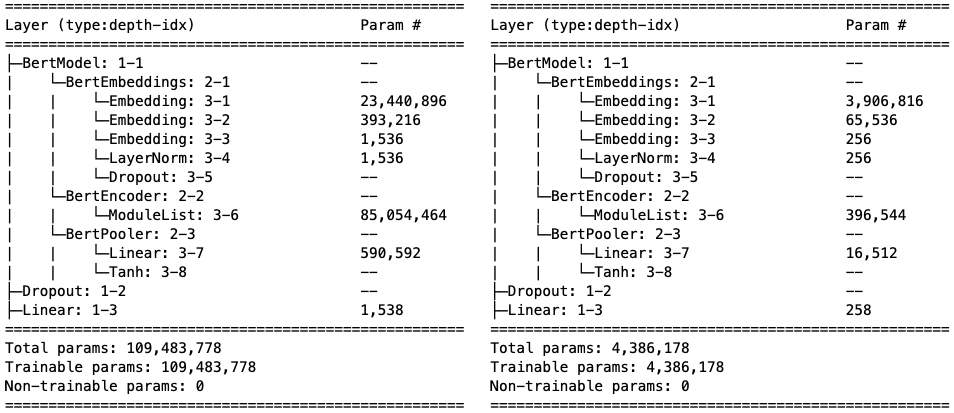
\includegraphics[width=15cm]{figures/model-summary.png}
    \vspace*{-3mm}
    \caption{A summary of the BERT Base (left) and BERT Tiny (right) models for comparison in terms of the layers used and number of parameters. This is based on the models from Hugging Face.}
    \label{fig: model_summary}
\end{figure}

\section{Data tokenisation}
The tokenization process is required for appropriate preparation of input data for use by BERT and its variants. The tokenization process\footnote{\url{https://huggingface.co/docs/datasets/use_dataset}} involves dividing the input text into tokens based on a predefined set of rules. These tokens are subsequently transformed into numerical representations and tensors, along with any extra inputs needed by the model. Tokens in general could be words, subwords, phrases or even characters. There are various approaches to tokenization and the methods used by each of the models in the scope of the experiments are indicated in Table \ref{tab: model_dtls}. The \texttt{transformers} library provides relevant methods to tokenize the input tweets. The library includes model-specific tokenizers such as, \texttt{BertTokenizer}\footnote{\url{https://huggingface.co/docs/transformers/v4.21.3/en/model_doc/bert#transformers.BertTokenizer}} or \texttt{RobertaTokenizer}\footnote{\url{https://huggingface.co/docs/transformers/v4.21.3/en/model_doc/roberta#transformers.RobertaTokenizer}} while models like BERT-tiny leverage existing ones. For the experiments, the \texttt{AutoTokenizer}\footnote{\url{https://huggingface.co/docs/transformers/v4.21.3/en/model_doc/auto#transformers.AutoTokenizer}} has been used which conveniently selects the appropriate tokenizer relevant for the model in use.

\subsection{Choice of settings}
Prior to applying tokenization, the settings for padding and truncation\footnote{\url{https://huggingface.co/docs/transformers/pad_truncation}} are chosen to ensure the varying input length will still result in rectangular tensors. The parameter, \texttt{max\_length} determines the maximum number of tokens for each input, \texttt{padding} controls the type of padding and \texttt{truncation} allows to truncate input to a pre-determined number of tokens.\newline

\begin{figure}[htbp]
    \centering
    \captionsetup{font=small}
    \begin{subfigure}[b]{0.48\textwidth}
        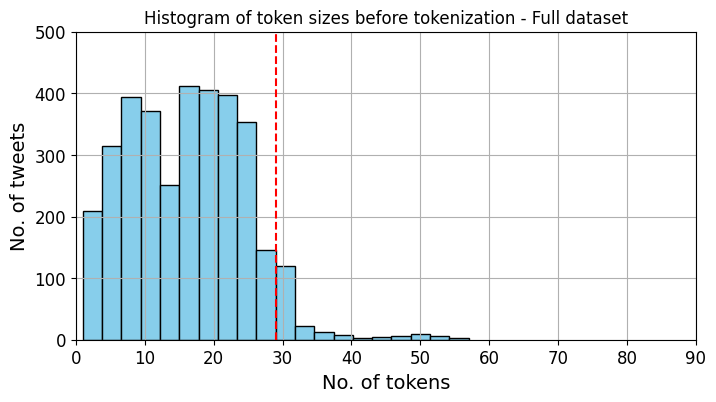
\includegraphics[width=\textwidth]{figures/token_hist.png}
        \caption{Before tokenization}
        \label{fig: token_hist}
    \end{subfigure}
    \hfill
    \begin{subfigure}[b]{0.48\textwidth}
        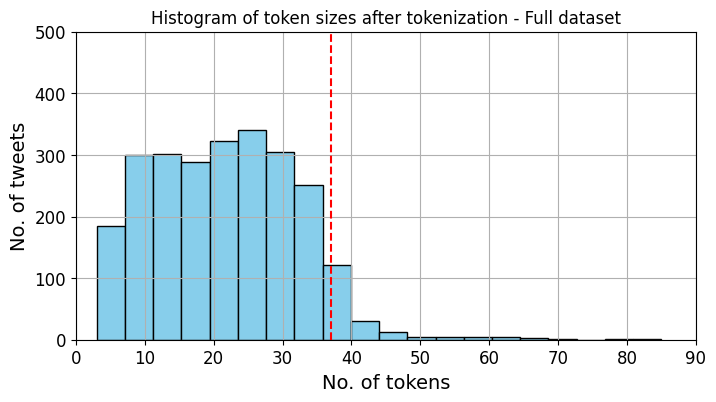
\includegraphics[width=\textwidth]{figures/token_pp_hist.png}
        \caption{After tokenization}
        \label{fig: token_pp_hist}
    \end{subfigure}
    \caption{The token count distribution for the full dataset of 3,449 tweets before and after tokenization with the red dashed line indicating 95\% coverage of tweets. BertTokenizer is used here.}
    \label{fig: bef_aft_token}
\end{figure}

The distribution of the number of tokens in the tweets from the pre-processed data from \cite{preotiuc-pietro_automatically_2019,jinModelingSeverityComplaints2021} before applying the model-specific tokenization is shown in Figure \ref{fig: token_hist}. Over 95\% of the tweets have 29 tokens or less. Using the BertTokenizer as an example, from Figure \ref{fig: token_pp_hist} it was found about 37 tokens are required to comprehensively cover 95\% of the tweets. The other tokenizers require between 35 and 43 tokens to cover the same percentage (refer Appendix \ref{sec: apdxa_token_dist}). This analysis assists in the decision on the appropriate \texttt{max\_value} for the tokenizer. A value of 50 ensures coverage of over 99\% of the tweets completely for all the tokenizers. This when used in conjunction with \texttt{truncation=True}, sets the maximum number of tokens for each input tweet to 50. Anything that follows is truncated and not used for training or inference. Additionally, since the dataset includes shorter tweets with resulting tokens less than 50, \texttt{padding} is set to \emph{'max\_length'} to apply padding up to 50 tokens.


\subsection{Tokenisation example}
An example tweet from the input data is shown in \textbf{A} below. The pre-processing applied by \cite{preotiuc-pietro_automatically_2019,jinModelingSeverityComplaints2021} results in punctuation as separate tokens, e.g. 'again' and '.'. The hashtags are retained as single tokens. After applying tokenisation using the \texttt{BertTokenizer}, the data is converted into a list of input IDs representing their reference into the model's vocabulary as shown in \textbf{B}. To better understand the effect of tokenization, \textbf{C} shows the decoded input from \textbf{B}. The tokenizer adds special tokens, \texttt{[CLS]} - classification token for the beginning of an input sequence, \texttt{[SEP]} - separator token to separate input sequences and \texttt{[PAD]} - padding token. Aside from this, punctuation is combined with the word for 'again.'. In the case of hashtags, the '\#' symbol has been separated out as a token.\\

\textbf{A - Tweet from input dataset}\newline

\begin{adjustbox}{minipage={\textwidth},fbox}
    \texttt{love it when i almost die rear ended by a semi cause my jeep turns off again
        . one day they will fix it \#jeepsucks \#chrysler}
\end{adjustbox} \newline\newline

\textbf{B - Encoding the input}\newline

\begin{adjustbox}{minipage={\textwidth},fbox}
    \texttt{[101, 2293, 2009, 2043, 1045, 2471, 3280, 4373, 3092, 2011, 1037, 4100, 3426,
                2026, 14007, 4332, 2125, 2153, 1012, 2028, 2154, 2027, 2097, 8081, 2009, 1001,
                14007, 6342, 10603, 1001, 17714, 102, 0, 0, 0, 0, 0, 0, 0, 0, 0, 0, 0, 0, 0,
                0, 0, 0, 0, 0]}
\end{adjustbox} \newline\newline

\textbf{C - Decoding the tokenized input}\newline

\begin{adjustbox}{minipage={\textwidth},fbox}
    \texttt{[CLS] love it when i almost die rear ended by a semi cause my jeep turns off
        again. one day they will fix it \# jeepsucks \# chrysler [SEP] [PAD] [PAD] [PAD]
            [PAD] [PAD] [PAD] [PAD] [PAD] [PAD] [PAD] [PAD] [PAD] [PAD] [PAD] [PAD] [PAD]
            [PAD] [PAD]}
\end{adjustbox}\\ \\

\section{Experiment set 1: Predictive performance comparison of BERT variants}
In the first experiment, the objective is to identify which of the models performs the best for the text classification task of complaint identification. Additionally, the relative performance of the models and the inference time will be analysed to assess how the model size impacts these aspects. A nested cross-validation approach will be used to experiment finetuning the model with various learning rate hyperparameter values and calculate mean performance metrics on inference. All models in scope for the experiments are pre-trained, hence finetuning will be performed for the downstream complaints identification task.\\

The nested cross-validation approach utilized is adapted from \cite{preotiuc-pietro_automatically_2019}. The outer loop consists of 6 iterations and the inner loop of 4 iterations. Each outer loop includes a stratified split of the entire dataset into train (\textbf{a}) and test (\textbf{b}) datasets. Within the inner loop, \textbf{a} is further split into inner train and dev datasets using stratified split with each iteration, finetuning and validating on 1 of the 4 learning rates set for hyperparameter tuning. The best model from the inner loop is selected based on the F1 score on the dev dataset. This best model is used to perform inference using the test dataset, \textbf{b}. At the end of the 6 outer loop iterations, the mean of the performance metrics is calculated as the final metrics for that model. While \cite{preotiuc-pietro_automatically_2019} used 10 iterations for the outer loop, it has been restricted to 6 for the experiments considering significant variations were not observed on the metrics. This is likely due to the smaller size of the dataset and 6 stratified splits capturing sufficient variability in the input dataset.\\
\begin{table}[ht]
    \captionsetup{font=small}
    \small
    \centering
    \begin{tabularx}{\textwidth}{|X|c|}
        \hline
        \rowcolor[gray]{0.7}
        \textbf{Parameter}        & \textbf{Value}           \\
        \hline
        Outer loop iterations     & 6                        \\
        \rowcolor[gray]{0.9}
        Inner loop iterations     & 4                        \\
        Random Seed               & 2023                     \\
        \hline
        \hline
        \rowcolor[gray]{0.7}
        \textbf{Hyperparameter}   & \textbf{Value}           \\
        \hline
        No. of Epochs             & 4                        \\
        \rowcolor[gray]{0.9}
        Learning Rate             & [1e-5, 5e-6, 5e-5, 3e-5] \\
        All other hyperparameters & Model defaults           \\
        \hline
    \end{tabularx}
    \caption{The choice of key parameters and hyperparameters used for experiment set 1.}
    \label{tab: exp1_params}
\end{table}

The key choices for the experiments including that of the hyperparameters are described in Table \ref{tab: exp1_params}. For the stratified split, the \texttt{StratifiedKFold} function from \texttt{sklearn} library is used. This results in approximately 2874 and 575 tweets for the outer loop's train and test datasets and 2155 and 719 tweets for the inner loop's train and dev datasets. The number of epochs is set to 4 in line with official documentation for BERT\footnote{\url{https://github.com/google-research/bert}} where they use between 2 and 4 epochs for the various downstream tasks. The learning rate includes the default rate used by the models as well as a range of alternate values. All other hyperparameters take on their default values for the models as defined in the \texttt{transformers} library.\\

For the predictive performance metrics, precision, recall, accuracy, F1 and Area under the ROC Curve (AUC) scores are computed for both the inner loop's validation as well as the outer loop's testing. Further, the final metrics for each model are based on each of the mean metrics from the 6 outer loop iterations. Additionally, the samples per second and steps per second are captured for each of the models during the inference phase to analyse the time taken for inference in relation to the model size.

\section{Experiment set 2: Cross-domain predictive performance comparison}
Cross-domain experiments are conducted to understand how the performance of finetuned models varies as the volume, domain and class balance of the tweets change.  This approach also offers an avenue to assess any linguistic variations among complaints across different domains and their consequent effects on the classification performance. \\

For the experiments, the best-performing model from the first experiment is utilised. The tweets for each of the 9 domains are used for training separately with tweets from every other domain used for testing. Additionally, each domain is used for testing while training is based on all tweets except the domain used for testing. Stratified split is applied on the training dataset for each domain using the \texttt{StratifiedKFold} function from \texttt{sklearn} library for 3 iterations of finetuning. At the end of each iteration, inference is performed on the testing data.  The number of epochs remains at '4', similar to experiment set 1 while the learning rate used is the best learning for the selected model from experiment set 1. All other hyperparameters are the model defaults. The parameters and hyperparameters used for the experiment are listed in Table \ref{tab: exp2_params}.\\

In this set of experiments, only the most effective model identified from the previous experiment is utilised. The model is finetuned using tweets belonging to one domain at a time while testing is performed for each of the remaining domains separately and performance recorded. Additionally, each domain is tested on a  model which is finetuned on all tweets except the domain used for testing.\\

To ensure the balance of classes is maintained for the training and evaluation sets, a stratified split is applied using the \texttt{StratifiedKFold} function from the \texttt{sklearn} library. This process is repeated for three iterations of finetuning. Following each iteration, the model's performance is evaluated through inference on the testing data. The experiment maintains a consistent number of epochs of 4, similar to the first experiment. The learning rate is determined by the optimal value identified in the initial experiment for the selected model. All other hyperparameters follow the model's default settings. For details of the parameters and hyperparameters employed in this experiment, please refer to Table \ref{tab: exp2_params}.

\begin{table}[ht]
    \captionsetup{font=small}
    \small
    \centering
    \begin{tabularx}{\textwidth}{|X|c|}
        \hline
        \rowcolor[gray]{0.7}
        \textbf{Parameter}        & \textbf{Value}                       \\
        \hline
        No. of iterations         & 3                                    \\
        \rowcolor[gray]{0.9}
        Random Seed               & 2023                                 \\
        \hline
        \hline
        \rowcolor[gray]{0.7}
        \textbf{Hyperparameter}   & \textbf{Value}                       \\
        \hline
        No. of Epochs             & 4                                    \\
        \rowcolor[gray]{0.9}
        Learning Rate             & Best learning rate from experiment set 1 \\
        All other hyperparameters & Model defaults                       \\
        \hline
    \end{tabularx}
    \caption{The choice of key parameters and hyperparameters used for experiment set 2. Refer to the Chapter on results for the model and learning rate used for this experiment. }
    \label{tab: exp2_params}
\end{table}
For each iteration and combination of domains for finetuning and testing, the prediction performance metrics are calculated for precision, recall, accuracy, F1, and AUC. At the end of the third iteration, the mean of the metrics is calculated. The results and findings from this set of experiments are presented in Chapter 4.

\section{Ethical, Professional and Legal Issues}
The data used for the experiments were created by \cite{preotiuc-pietro_automatically_2019} and further enhanced with complaints severity type annotation by \cite{jinModelingSeverityComplaints2021}. This data is anonymised and is available in the public domain\footnote{\url{ https://archive.org/details/complaint_severity_data}}. No additional data has been collected for the experiments conducted for this project. To ensure the appropriate compliance with the ethical review requirements of the University of Sheffield, a self-declared ethics review application with reference number 054854 was raised and subsequently approved by the University Research Ethics Committee.

\chapter{Results and discussion}

\section{Data exploration}
As described in Chapter 3, the data for the experiments is taken from Twitter. It was extracted and pre-processed by \cite{preotiuc-pietro_automatically_2019} and further enhanced with the labels for complaint severity by \cite{jinModelingSeverityComplaints2021}. What follows are the key findings from the exploratory data analysis performed. Some minor differences in the distribution of the tweets across the domains are observed between the latest version of the dataset available in the public domain\footnote{\url{https://archive.org/details/complaint_severity_data}} and the distribution described in the original paper. Since the variations are minor (0.5 to 2\%), any potential impact on the model performance should be insignificant in the context of the objectives of the experiments. Refer \ref{sec: apdxa_fulldataset} for the full breakdown of the dataset used here.

\subsection{Domain and class distribution}
\begin{figure}[htb]
    \centering
    \captionsetup{font=small}
    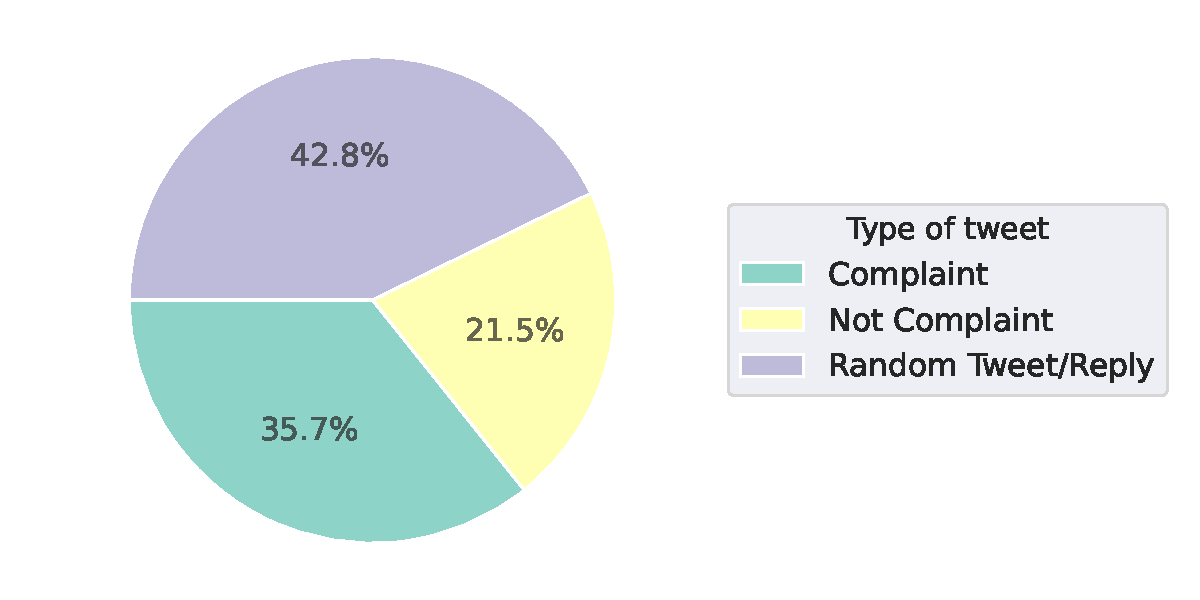
\includegraphics[width=9cm]{figures/compl_non_random_dist.pdf}
    \vspace*{-3mm}
    \caption{Illustrates the distribution of tweets categorised as 'complaints' and 'not complaints', with random 'tweets / replies' shown separately.}
    \label{fig: compl_non_random_dist}
\end{figure}


All tweets categorised as complaints are assigned \texttt{label:1}, while tweets that do not constitute complaints are assigned \texttt{label:0}. In terms of class distribution, the dataset is skewed towards 'not complaint' tweets, as depicted in Figure \ref{fig: compl_non_random_dist}, where \texttt{label:1} represents 35.7\% and \texttt{label:0} represents 64.3\% of the dataset. Random tweets and replies with \texttt{label:0} were added by the authors of \cite{preotiuc-pietro_automatically_2019} to ensure a more representative dataset. This approach aligns with the real-world scenario where complaint-related posts form a smaller proportion within an organization's social media tweets and posts. Additionally, this strategy has the potential to enhance the model's ability to generalize effectively during the finetuning process.\\

\begin{figure}[htbp]
    \centering
    \captionsetup{font=small}
    \begin{subfigure}{0.49\textwidth}
        \centering
        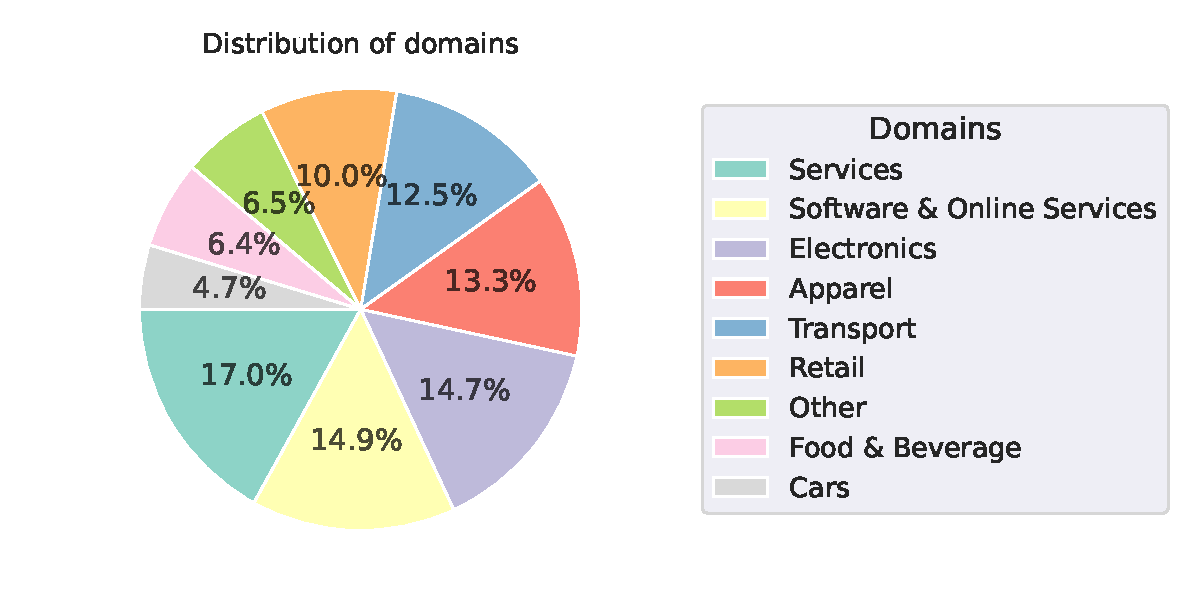
\includegraphics[width=\linewidth]{figures/domain_dist.pdf}
        \caption{Proportion of each domain}
        \label{fig: domain_dist_pct}
    \end{subfigure}
    \hfill
    \begin{subfigure}{0.49\textwidth}
        \centering
        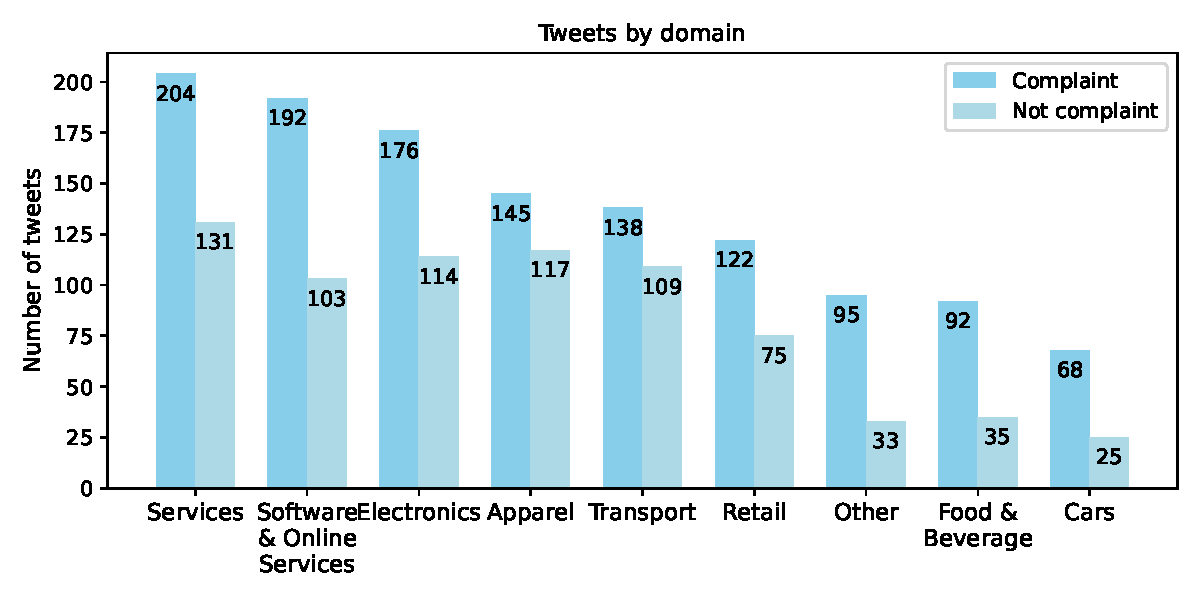
\includegraphics[width=\linewidth]{figures/domain_counts_bar_norandom.pdf}
        \caption{No. of tweets for each domain}
        \label{fig: domain_dist_count}
    \end{subfigure}
    \caption{Shows the distribution of the domains used in the dataset}
    \label{fig: compl_main_dist}
\end{figure}

The dataset comprises domains encompassing both complaint-related tweets and non-complaint tweets. Figure \ref{fig: domain_dist_pct} illustrates the distribution of domains, with the top 3 categories being services, software, and electronics, collectively constituting nearly 50\% of the tweets. A key observation from Figure \ref{fig: domain_dist_count} is the prevalent class imbalance within most domains, accompanied by relatively low tweet volumes within each domain. The implications of these observations on predictions are analyzed in Experiments set 2 and elaborated upon later in this chapter.

\begin{figure}[htbp]
    \centering
    \captionsetup{font=small}
    \begin{subfigure}{0.49\textwidth}
        \centering
        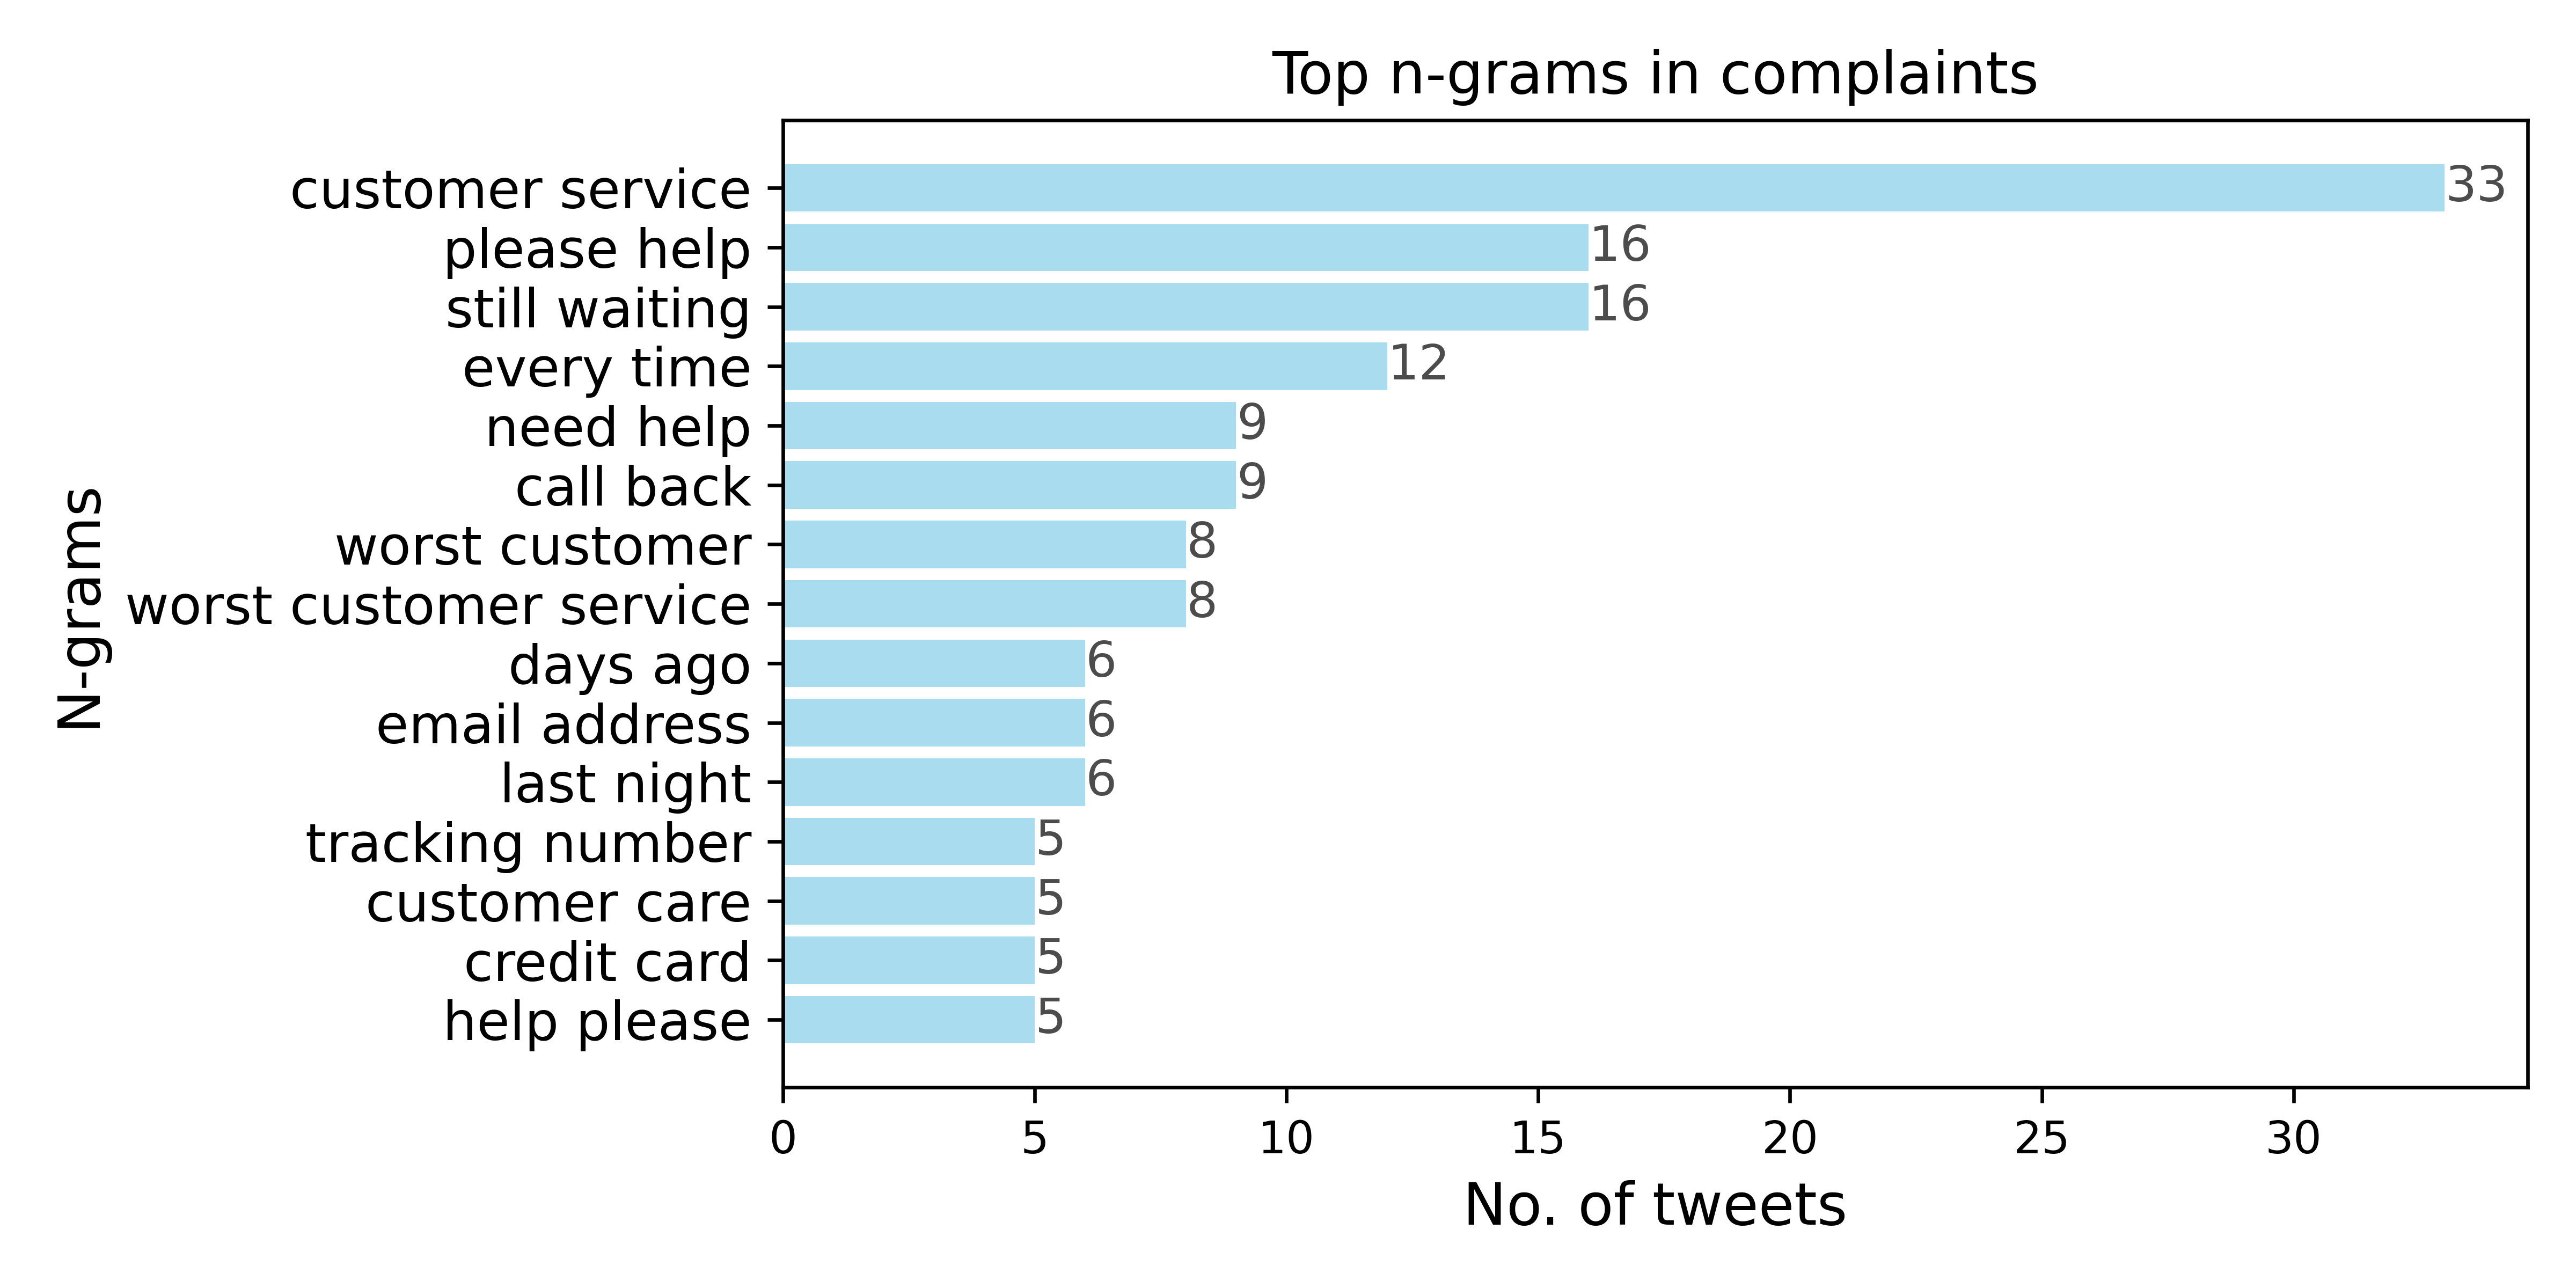
\includegraphics[width=\linewidth]{figures/top_ngram_horiz_bar.png}
        \caption{Top n-grams}
        \label{fig: top_ngrams}
    \end{subfigure}
    \hfill
    \begin{subfigure}{0.49\textwidth}
        \centering
        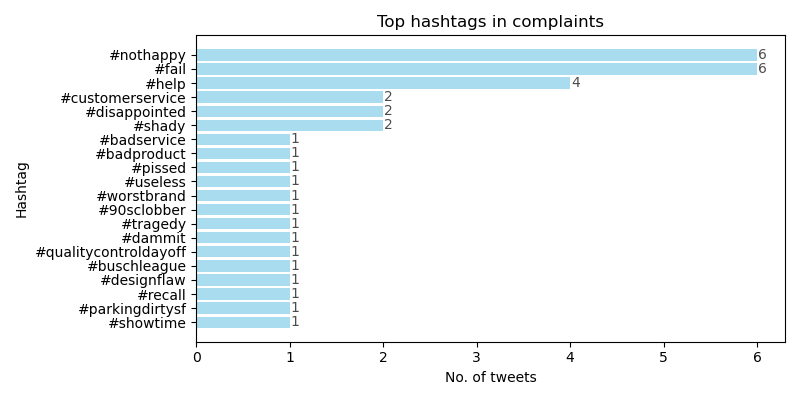
\includegraphics[width=\linewidth]{figures/top_hash_horiz_bar.png}
        \caption{Top hashtags}
        \label{fig: top_hashtags}
    \end{subfigure}
    \caption{Top phrases as n-grams(excl. unigrams) and hashtags in the complaint tweets.}
    \label{fig: top_ngrams_hashtags}
\end{figure}

\subsection{Linguistic analysis}
Delving deeper into the language used in Twitter complaints, the top phrases are analysed by extracting n-grams. As depicted in Figure \ref{fig: top_ngrams}, common phrases in the complaint tweets either convey an exepectation for resolution (such as "please help" and "need help") or express frustration (like "still waiting," "worst customer service," and "call back"). Others cover  broader customer service themes (for instance, "tracking number" and "customer care"). To elaborate further, sample tweets with these phrases are shown below. They showcase various characteristics previously discussed, including instances of Face Threatening Acts, feelings of betrayal, altruistic behaviour (warning others), as well as elements like sarcasm. These findings align with the definition of a complaint and the intentions of the speaker as outlined in previous chapters.\\

\textbf{Examples for expectation of rectification}
\begin{quote}
    \textit{"hey chrysler cares i'm the one with the 2011 200 \textbf{need help} with the heating . inside the car it's really strange"}
\end{quote}
\begin{quote}
    \textit{"can someone \textbf{please help} me ? i've already sent a dm ."}
\end{quote}
\textbf{Examples for expression of frustration}
\begin{quote}
    \textit{"\textbf{worst customer service} experience with <user> <user> <user> . never been treated with such contempt"}
\end{quote}
\begin{quote}
    \textit{"on hold with <user> an hour just to get told to \textbf{call back} another day . hell yeah"}
\end{quote}
\begin{quote}
    \textit{"\textbf{worst customer service} to-date <user> in greensboro off wendover . avoid this place and let's show them we have other choices . \#otherchoices"}
\end{quote}

Examination of the hashtags within the complaint tweets as shown in Figure \ref{fig: top_hashtags} points to their usage predominantly as a means of conveying frustration. Hashtags such as \texttt{\#nothappy}, \texttt{\#fail}, and \texttt{\#disappointed} are examples. Consequently, in addition to expressing dissatisfaction, these hashtags also communicate negative sentiments. Apart from these particular types of hashtags, various brand-specific or product-specific hashtags are used. As per Twitter\footnote{\url{https://help.twitter.com/en/using-twitter/how-to-use-hashtags#}}, users utilize the symbol "\#" (hashtag) preceding a keyword or phrase significant to the context in their tweet to classify those tweets, facilitating their visibility in Twitter searches. Clicking or tapping on a hashtagged term within any message reveals additional tweets containing the same hashtag. Hashtags can be inserted at any point within a tweet. Frequently, words marked with hashtags that attain significant popularity transform into trending topics. \\

However, the volume of tweets which include hashtags, particularly in the context of complaints is relatively low. Out of a total of 459 tweets, only 149 complaint tweets incorporate hashtags, constituting roughly 12\% of all complaint-related tweets. When excluding random tweets and replies, the tweets that are not complaints containing hashtags amount to only 67 instances. There is an average of 1.56 hashtags in tweets containing at least one. While the inclusion of hashtags may offer some assistance to the predictions by the models, their overall impact on the fine-tuning process could be quite limited due to their low prevalence in the dataset.\\

\subsection{Sentiment analysis}
\begin{figure}[htb]
    \centering
    \captionsetup{font=small}
    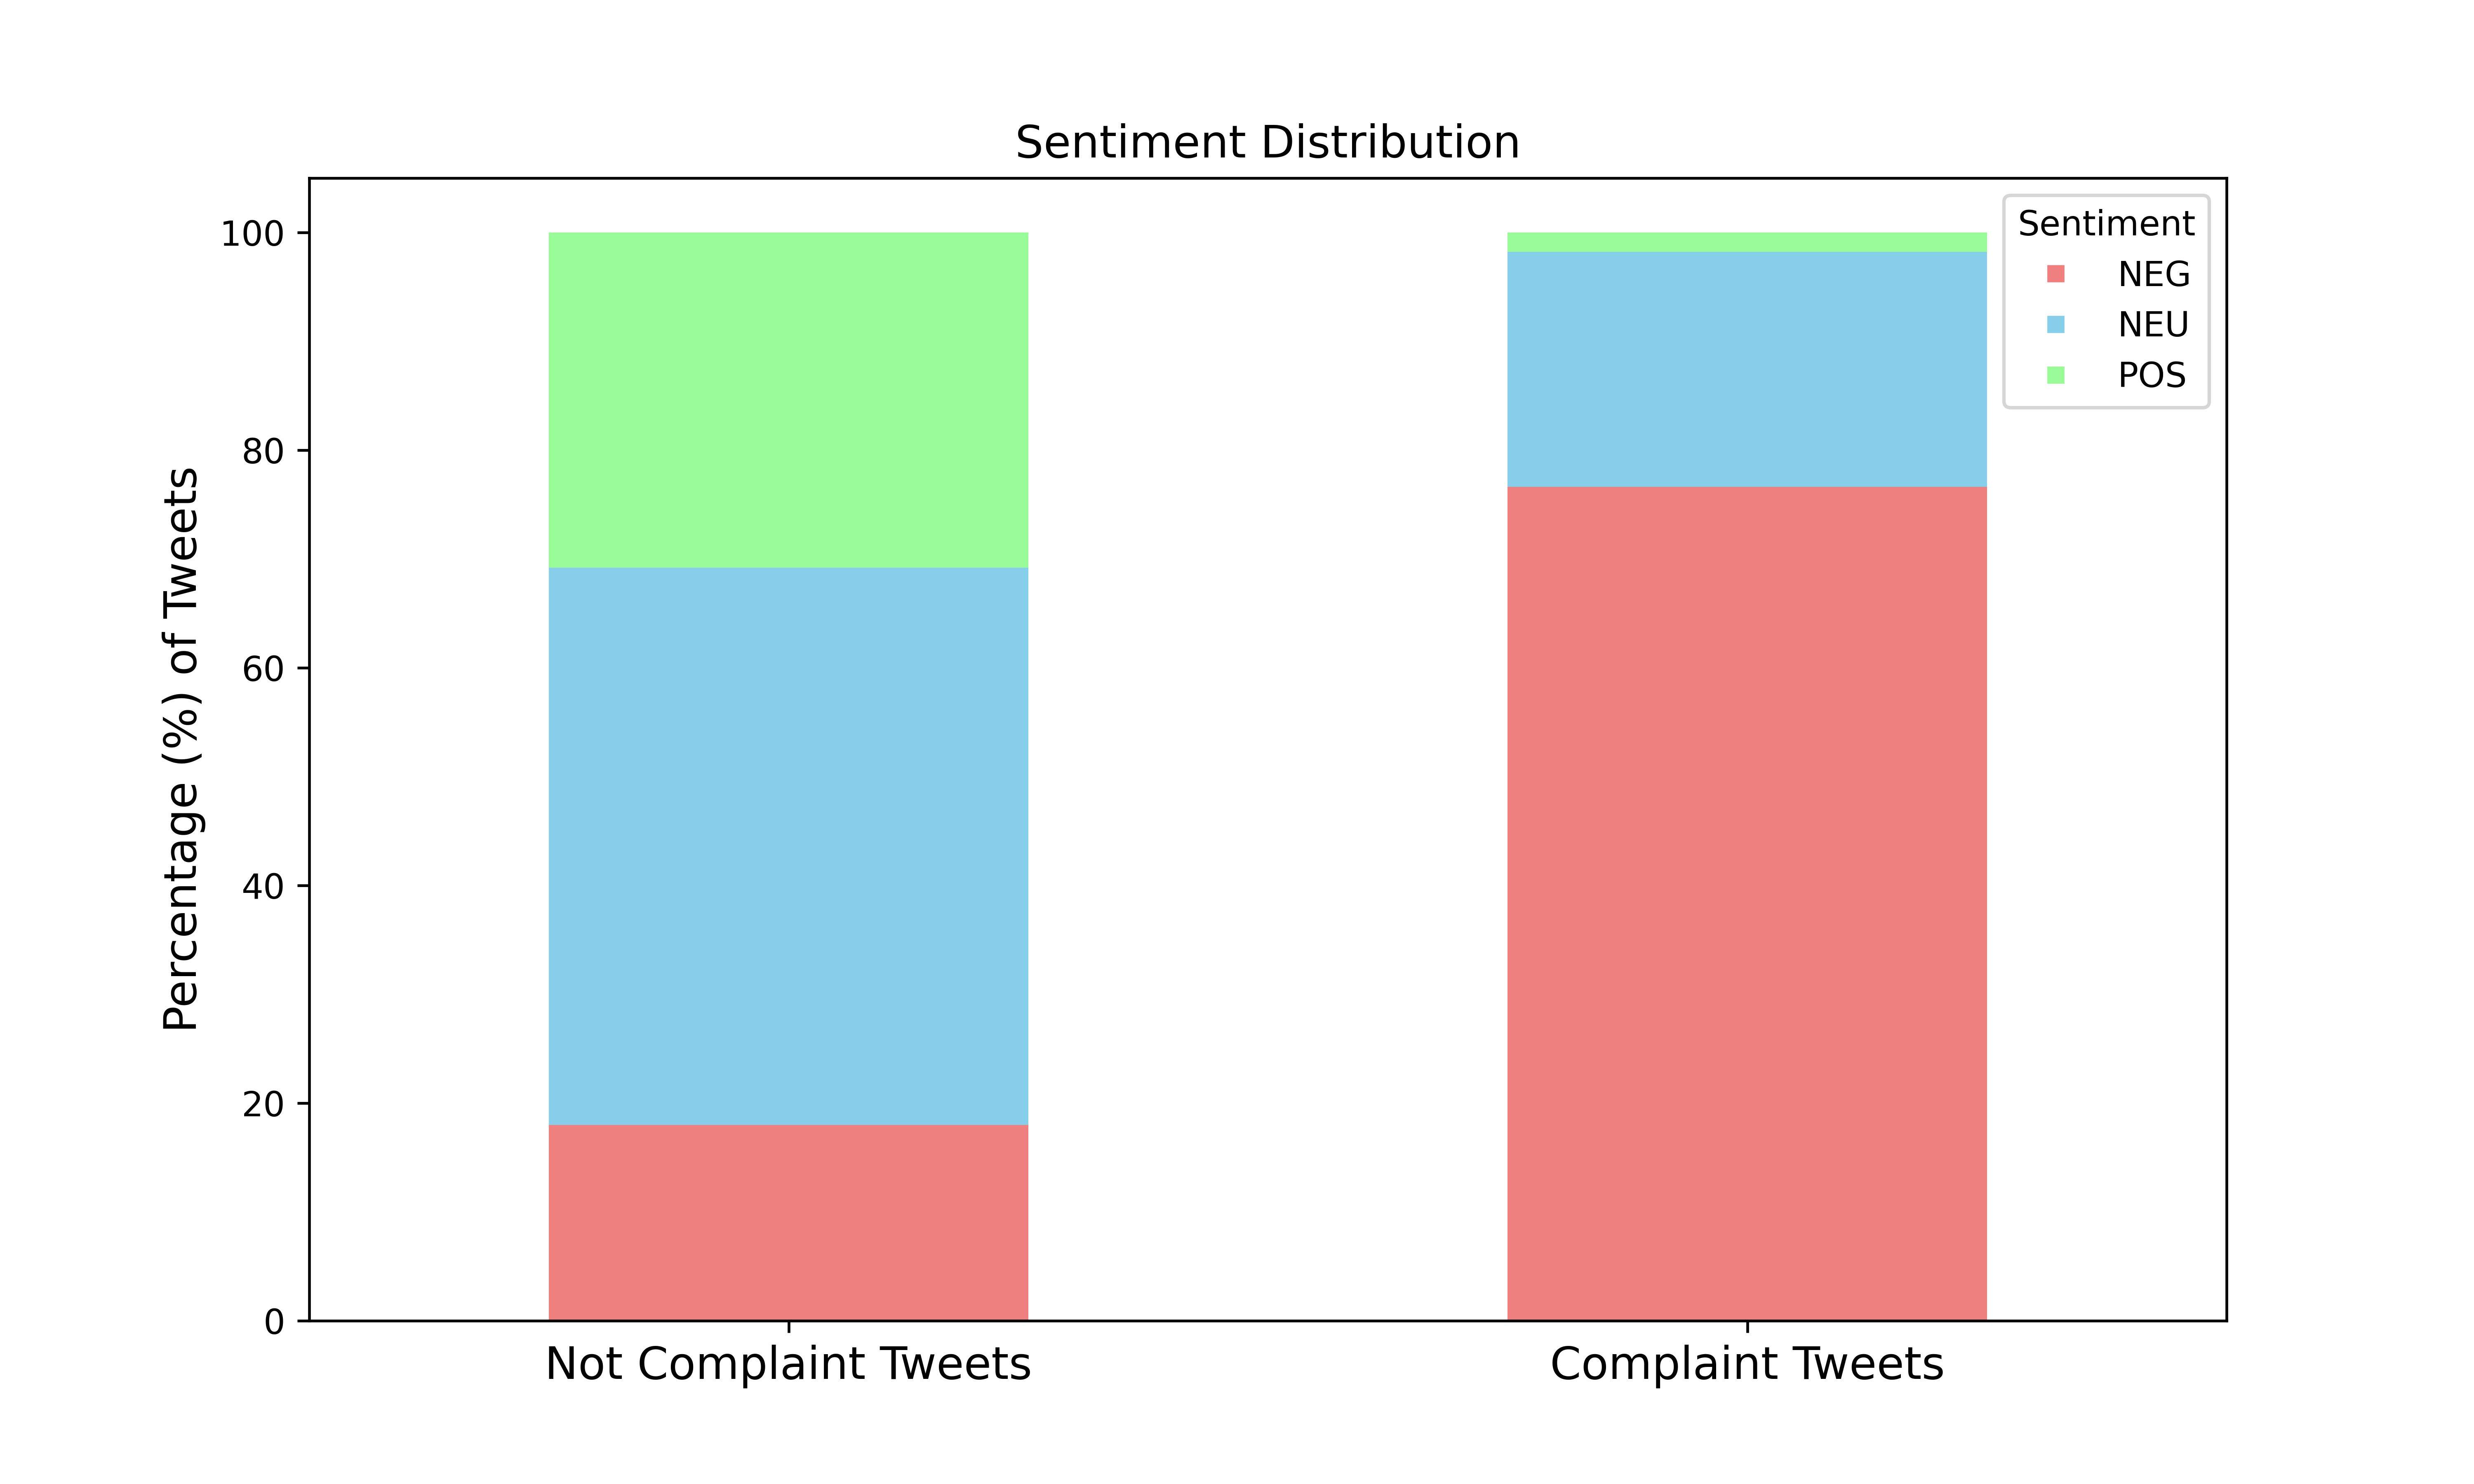
\includegraphics[width=12cm]{figures/sentiment.png}
    \vspace*{-3mm}
    \caption{Distribution of positive, negative and neutral sentiments in the tweets.}
    \label{fig: sentiment}
\end{figure}

The act of complaining typically involves conveying a sense of negativity. Sentiment analysis was conducted on the dataset using  pysentimiento's library \cite{perezPysentimientoPythonToolkit2021} and the results are in Figure \ref{fig: sentiment}. As expected, the majority of complaint-related tweets convey some form of negative sentiment, while approximately a quarter of them exhibit a neutral sentiment. A few examples of such neutral sentiment tweets are as follows: \textit{"anyone know what's up with the geforce 500 series 580 gpx driver 275.33"} and \textit{"hi m order is 913181 did you revise the money ? if you did .. how about the shipping ?"}. These instances appear to involve raising a complaint while simultaneously posing a question that doesn't overtly express negative sentiment. While an undercurrent of dissatisfaction is evident, the situation has not escalated to the point requiring language which explicitly expresses negative sentiment.\\

Next, the small number of positive tweets among the complaints were analysed. It was found they mostly involved sarcasm or where the consumer was expressing their liking for a product with the hope this could quicken the resolution process. Some of the example tweets for these scenarios are: \textit{"hello i have a 2012 impreza and i love it . my driver seat back is broken down after 1 year and 12000 miles 32000 total 2nd owner"} and \textit{"i love waiting at mcdonalds for 15 minutes just for some semi-good ice cream <url>"}. For tweets that were not complaints, the majority of them expressed neutral or positive sentiments.

\subsection{Key statistics}
% key statistcis table
\begin{table}[htbp]
    \captionsetup{font=small}
    \small
    \centering
    \begin{tabularx}{\textwidth}{|l|X|X|X|X|}
        \hline
        \rowcolor[gray]{0.7}
        \textbf{Statistic}              & \textbf{All Tweets} & \textbf{Complaints} & \textbf{Not Complaints} & \textbf{Random} \\
        \hline
        Number of tweets                & 3449                & 1232                & 742                     & 1475            \\
        \rowcolor[gray]{0.9}
        Number of unique tweets         & 3395                & 1232                & 737                     & 1427            \\
        \hline
        \hline
        Max tweet length (char.)        & 297                 & 297                 & 266                     & 144             \\
        \rowcolor[gray]{0.9}
        Min tweet length (char.)        & 1                   & 7                   & 6                       & 1               \\
        Mean tweet length (char.)       & 77.8                & 96.7                & 70.2                    & 65.8            \\
        \rowcolor[gray]{0.9}
        Median tweet length (char.)     & 79.0                & 98.0                & 68.0                    & 63.0            \\
        Standard Deviation tweet length & 41.4                & 40.5                & 38.9                    & 37.5            \\
        \hline
        \hline
        Total number of tokens          & 55169               & 24260               & 10839                   & 20070           \\
        \rowcolor[gray]{0.9}
        No. of unique tokens            & 7937                & 4031                & 2558                    & 4386            \\
        Maximum tokens                  & 57                  & 57                  & 55                      & 39              \\
        \rowcolor[gray]{0.9}
        Minimum tokens                  & 1                   & 2                   & 1                       & 1               \\
        Mean tokens                     & 16.0                & 19.7                & 14.6                    & 13.6            \\
        \rowcolor[gray]{0.9}
        Median tokens                   & 16.0                & 20.0                & 14.0                    & 13.0            \\
        Standard Deviation for tokens   & 8.6                 & 8.4                 & 8.0                     & 8.0             \\
        \hline
        \hline
        Mean punctuation count          & 3.4                 & 3.9                 & 2.7                     & 3.3             \\
        \hline
    \end{tabularx}
    \caption{Statistics of tweets in the dataset.}
    \label{tab: tweets_statistics}
\end{table}

Finally, examining some of the key statistical measures from the tweets dataset in Table \ref{tab: tweets_statistics}, complaint tweets tend to exhibit a higher average tweet length, both in terms of characters (96.7) and tokens (19.7). In contrast, random tweets and replies have a token count lower by 30\%, while non-complaint tweets possess an average of 25\% fewer tokens than complaint tweets. This disparity may stem from individuals employing diverse linguistic expressions to express their dissatisfaction or disappointment, or to communicate a Face Threatening Act directed at the subject of the complaint.

\section{Experiment set 1 results: Comparision of model performance}
As described in the previous chapter, to compare the performance of the models a nested cross-validation approach was adopted. The cross-validation method finetuned the models using 4 learning rates, $l\:\epsilon\:[1e-5, 5e-6, 5e-5, 3e-5]$ with the best-performing model based on the F1 score being selected for the testing for each iteration of the outer loop. \\

\subsection{Best predictive performance}
The best-performing model was found to be BERTweet with a mean F1 score of 0.908 (sd: $\pm$0.01), accuracy of 0.934 (sd: $\pm$0.01) and ROC AUC of 0.931 (sd: $\pm$0.01) as shown in Table \ref{tab: model_mean_metrics}. Using F1 and AUC ROC scores for the assessment is more meaningful than using accuracy alone due to the class imbalance present in the dataset. BERTweet being pre-trained on a corpus of 850M tweets could be giving it an advantage in capturing the nuances of social media posts including informal language, typographic errors, use of slang and expressive lengthening and more specific characteristics of tweets such as the use of shorter messages, abbreviations and hashtags. From the experiments, 0.00003 was the best learning rate identified from the inner loop iterations for BERTweet Base and this is used for the experiments set 2, the results for which are detailed in the next section. RoBERTa was the next best performing model with an F1 of 0.879 (sd: $\pm$0.03), an accuracy of 0.914 (sd: $\pm$0.02) and AUC of 0.905(sd: $\pm$ 0.02). It was followed by BERT Base and DistilBERT with F1 scores of 0.865 (sd: $\pm$0.02) and 0.863 (sd: $\pm$0.02) respectively.

Table \ref{tab: model_mean_metrics} also includes the prediction metrics sourced from \cite{jin_complaint_2020}, enclosed within '[ ]', which serves as the established baseline performance for this task. Despite the variation in nested cross-validation configuration, as outlined in the preceding chapter, a level of preliminary comparison becomes feasible. In terms of F1 scores, RoBERTa shows marginal improvement, while BERT Base and ALBERT perform slightly worse. However, overall BERTweet provides the best predictive results for this task when compared to the baseline.\\

\begin{table}[htbp]
    \centering
    \small % Set font size to \small
    \begin{tabularx}{\textwidth}{|X|X|X|X|X|X|}
        \hline
        \rowcolor[gray]{0.7}
        \textbf{Model}                                  & \textbf{Accuracy} & \textbf{Precision} & \textbf{Recall} & \textbf{F1}    & \textbf{ROC AUC} \\
        \hline
        AlBERT Base v2                                  & 0.879 [0.859]     & 0.845 [0.848]      & 0.811 [0.846]   & 0.827 [0.846]  & 0.864            \\
        \rowcolor[gray]{0.9}
        \(\star\)\(\uparrow\) BERTweet Base             & \textbf{0.934}    & \textbf{0.897}     & \textbf{0.920}  & \textbf{0.908} & \textbf{0.931}   \\
        BERT Base uncased                               & 0.905 [0.88]      & 0.878  [0.871]     & 0.854  [0.873]  & 0.865 [0.87]   & 0.894            \\
        \rowcolor[gray]{0.9}
        \(\star\)\(\downarrow\) BERT Tiny & 0.772             & 0.701              & 0.627           & 0.662          & 0.739            \\
        \(\star\) DistilBERT Base uncased               & 0.903             & 0.872              & 0.860           & 0.863          & 0.894            \\
        \rowcolor[gray]{0.9}
        RoBERTa Base                                    & 0.914 [0.876]     & 0.886 [0.866]      & 0.873 [0.869]   & 0.879 [0.866]  & 0.905            \\
        \hline
    \end{tabularx}
    \caption{Mean prediction performance metrics for all models after nested cross-validation for finetuning and testing. The highest scores are in bold. \(\uparrow\) is the best performing and \(\downarrow\) is the worst performing model. \(\star\) models are included for deep-dive analysis. Where available, numbers in '[ ]' are the results from \cite{jin_complaint_2020}.}
    \label{tab: model_mean_metrics}
\end{table}

\subsection{Performance of smaller models}
Examining the smaller models characterized as lightweight based on their architecture and parameter count, DistilBERT emerges as the top performer, achieving an F1 score of 0.863 (sd: $\pm$0.02) and AUC of 0.894 (sd: $\pm$0.02). ALBERT follows suit with an F1 score of 0.827 (sd: $\pm$0.02) and AUC of (sd: $\pm$0.04). BERT Tiny, the smallest model employed in the experiments, exhibits a notable performance gap, achieving only an F1 score of 0.662 (sd: $\pm$0.04), which is lower by 27.6\% in comparison to BERTweet. This aligns with its low accuracy and AUC scores of 0.772 (sd: $\pm$0.02) and 0.739 (sd: $\pm$0.03) respectively. This points to a likely and significant performance penalty from the reduced model size. However, it is expected to perform better in the context of a knowledge distillation teacher \cite{turcWellReadStudentsLearn2019}, something that has not been tested here.\\

% Model size vs performance against BERTweet
\begin{figure}[htb]
    \centering
    \captionsetup{font=small}
    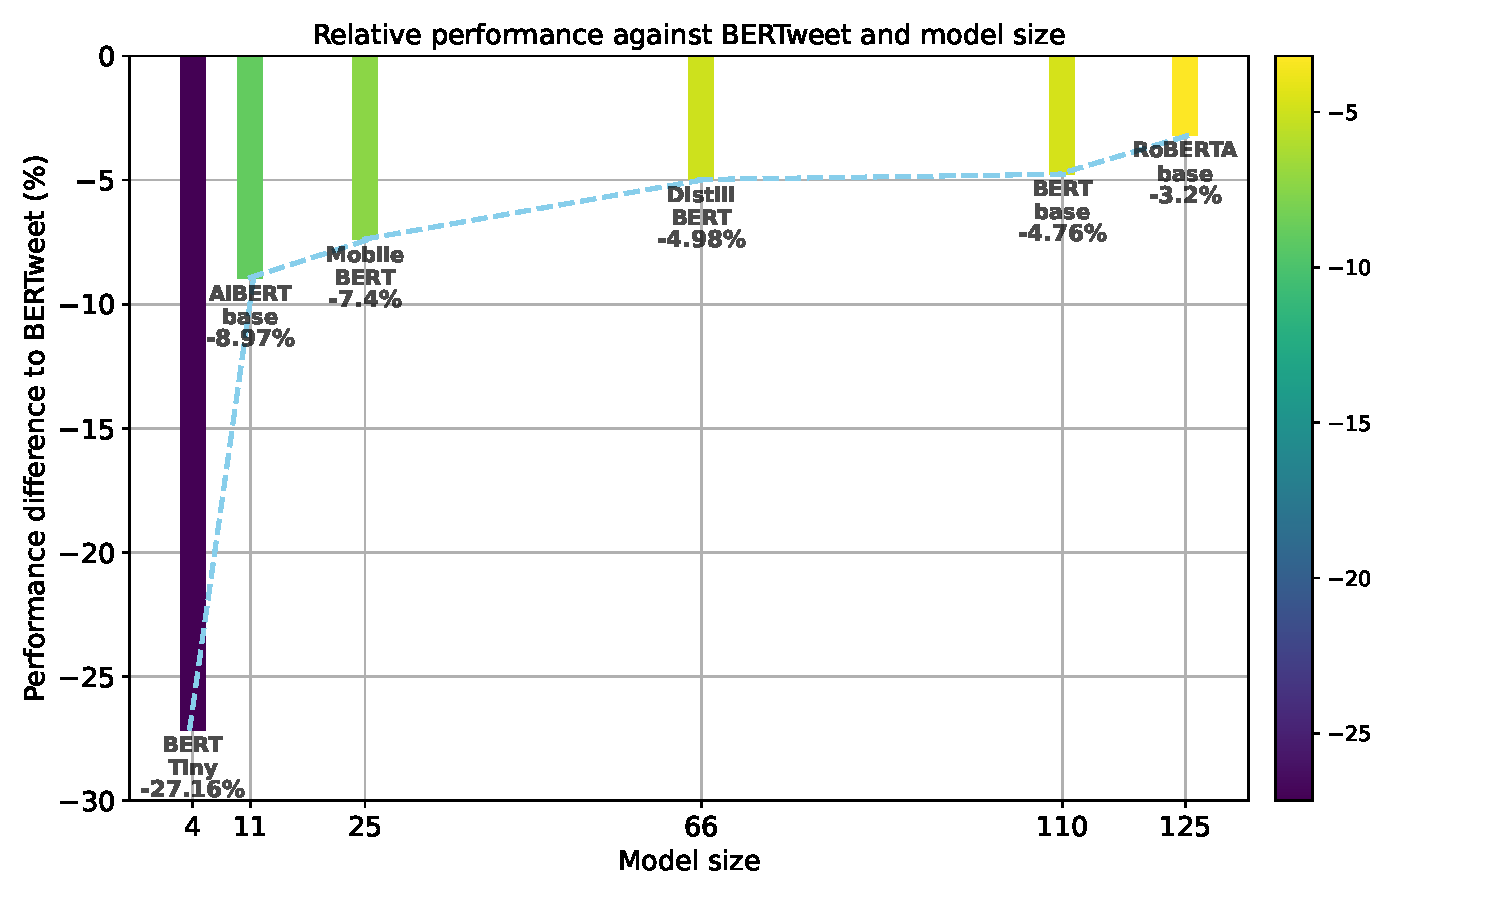
\includegraphics[width=12cm]{figures/model_size_vs_perf.pdf}
    \vspace*{-3mm}
    \caption{Relative performance of models against BERTweet and model sizes based on F1. BERTweet's model size is 110M.}
    \label{fig: model_size_vs_perf}
\end{figure}

% Relative performance table
\begin{table}
    \small
    \centering
    \begin{tabularx}{\textwidth}{|X|c|c|c|c|}
        \hline
        \rowcolor[gray]{0.7}
        \textbf{Model} & \textbf{F1} & \textbf{Model size} & \textbf{Train time} & \textbf{Inference time} \\
        \hline
        \textit{BERTweet}       & \textit{0.908}       & \textit{110M}                & \textit{87.19 s}             & \textit{0.987 s}                 \\
        \hline
        RoBERTa Base   & -3.2\%      & +13.6\%             & -4.5\%              & -1.6\%                  \\
        \rowcolor[gray]{0.9}
        BERT Base      & -4.8\%      & +0.0\%              & -10.7\%             & +1.2\%                  \\
        DistilBERT     & -5.0\%      & -40.0\%             & -50.7\%             & -43.3\%                 \\
        \rowcolor[gray]{0.9}
        ALBERT         & -9.0\%      & -90.0\%             & -40.3\%             & +22.8\%                 \\
        BERT Tiny      & -27.1\%     & -96.0\%             & -86.4\%             & -70.2\%                 \\
        \hline
    \end{tabularx}
    \caption{Comparison of key metrics of the models relative to BERTweet.}
    \label{tab: relative_comparison_metrics}
\end{table}

Figure \ref{fig: model_size_vs_perf} displays the relative variance in model performance when compared to BERTweet based on F1, alongside the corresponding model sizes or the number of parameters. Table \ref{tab: relative_comparison_metrics} expands on this by including the relative difference of the models compared to BERTweet in terms of model size, training time and inference time. Notably, ALBERT exhibits a relatively lower performance discrepancy of 8.9\%, considering the model size is significantly smaller by 90\%. DistilBERT demonstrates a performance deficit of merely 4.9\%, not far off from BERT Base while having a model size lower by 44\%. This could likely be due to the knowledge distillation and compression techniques applied during the pretraining phase, which could be playing a key role in enhancing DistilBERT's predictive capabilities \cite{sanhDistilBERTDistilledVersion2020}.\\

\subsubsection{Analyis of finetuning and inference time}

Next, the time required for inference and training (finetuning) is analysed and shown in Figure \ref{fig: mean_time_taken}. On average, the number of rows for the train, dev and test splits was 2155, 719 and 575. The training and inference were executed on a single NVIDIA RTX A4000 GPU with 16GB VRAM. BERT Tiny as expected has the lowest mean training and inference time. It is lower by over 85\% and 70\% for training and inference respectively as shown in Table \ref{tab: relative_comparison_metrics} when compared to BERTweet. DistilBERT follows next with lower train and inference times by 51\% and 43\%. For ALBERT the train time is lower than BERTweet by 40\%, while the inference time is slightly higher than BERT Base. ALBERT was designed to reduce the training time and memory footprint while lowering the inference time was not an explicit goal \cite{lanALBERTLiteBERT2020}. Hence these results seem to be in line with its architecture. 
% training and inference time bar chart
\begin{figure}[htbp]
    \centering
    \captionsetup{font=small}
    \begin{subfigure}{0.49\textwidth}
        \centering
        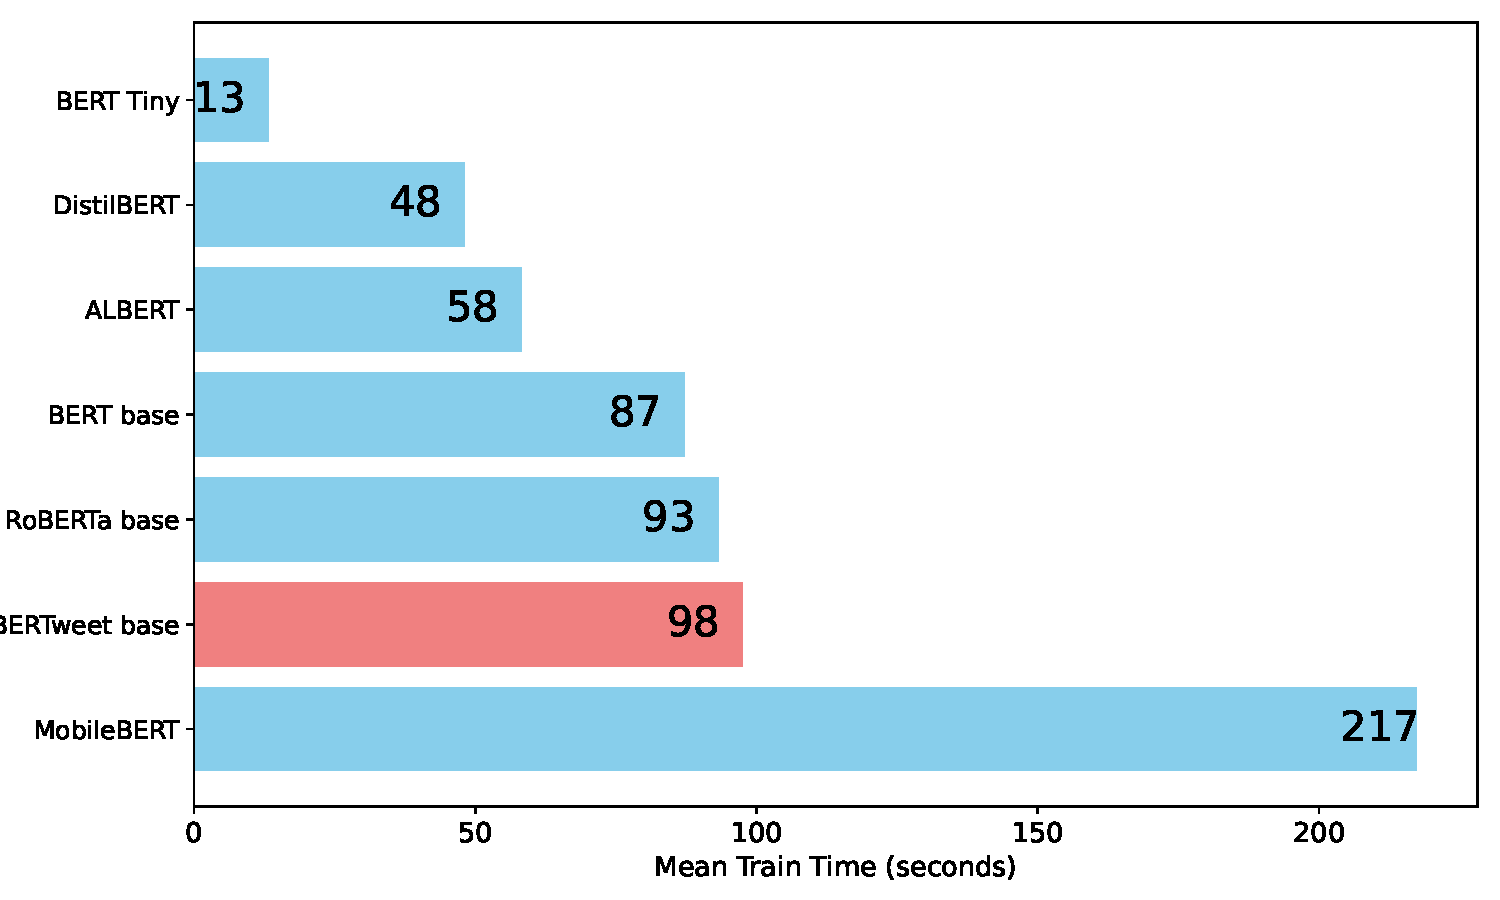
\includegraphics[width=\linewidth]{figures/mean_train_time.pdf}
        \caption{Mean training time.}
        \label{fig: mean_train_time}
    \end{subfigure}
    \hfill
    \begin{subfigure}{0.49\textwidth}
        \centering
        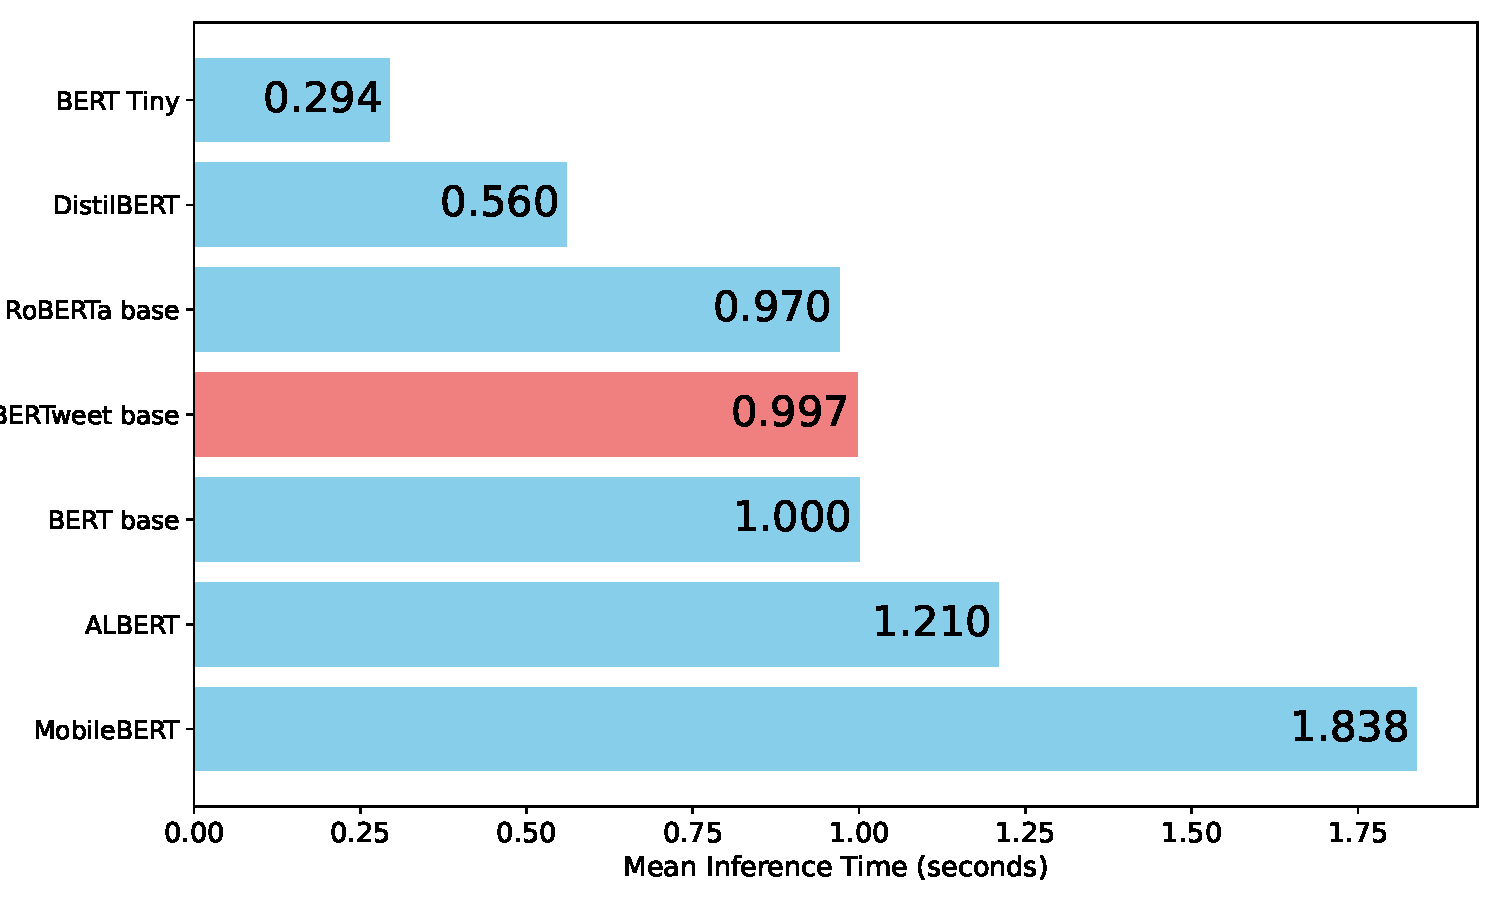
\includegraphics[width=\linewidth]{figures/mean_inference_time.pdf}
        \caption{Mean inference time}
        \label{fig: mean_inf_time}
    \end{subfigure}
    \caption{Mean time taken (in seconds) for finetuning and inference during experiments set 1. BERTweet with the best predictive model is highlighted in red.}
    \label{fig: mean_time_taken}
\end{figure}

\subsection{Deep-dive into the results}
To comprehend where the models are misclassifying, deep-dive analysis is carried out on the performance of select models. The overall best-performing model, BERTweet Base, the best-performing lightweight model, DistilBERT and the worst-performing model, BERT Tiny are chosen for this exercise. The scores from \ref{tab: model_mean_metrics} will be looked into in more detail along with the confusion matrix and sample misclassified tweets. The confusion matrix is based on the mean values from the 6 runs of inference carried out.\\
% Test loss table
\begin{table}[ht]
    \small
    \centering
    \begin{tabularx}{\textwidth}{|X|X|X|X|}
        \hline
        \rowcolor[gray]{0.7}
        \textbf{Test Run} & \textbf{BERTweet Base} & \textbf{DistilBERT} & \textbf{BERT Tiny} \\
        \hline
        1                 & 0.21701                & 0.22481             & 0.49180            \\
        \rowcolor[gray]{0.9}
        2                 & 0.20056                & 0.24783             & 0.50118            \\
        3                 & 0.23015                & 0.26190             & 0.48807            \\
        \rowcolor[gray]{0.9}
        4                 & 0.23572                & 0.25394             & 0.48178            \\
        5                 & 0.25255                & 0.30100             & 0.53076            \\
        \rowcolor[gray]{0.9}
        6                 & 0.17506                & 0.26712             & 0.48810            \\
        \hline
    \end{tabularx}
    \caption{Test loss from the inference phase for the 6 outer loop iterations for the 3 selected models.}
    \label{tab: test_loss}
\end{table}

% Deep dive confusion matrices and line graphs
\begin{figure}[!ht]
    \centering
    \captionsetup{font=small}
    \begin{subfigure}{0.45\linewidth}
        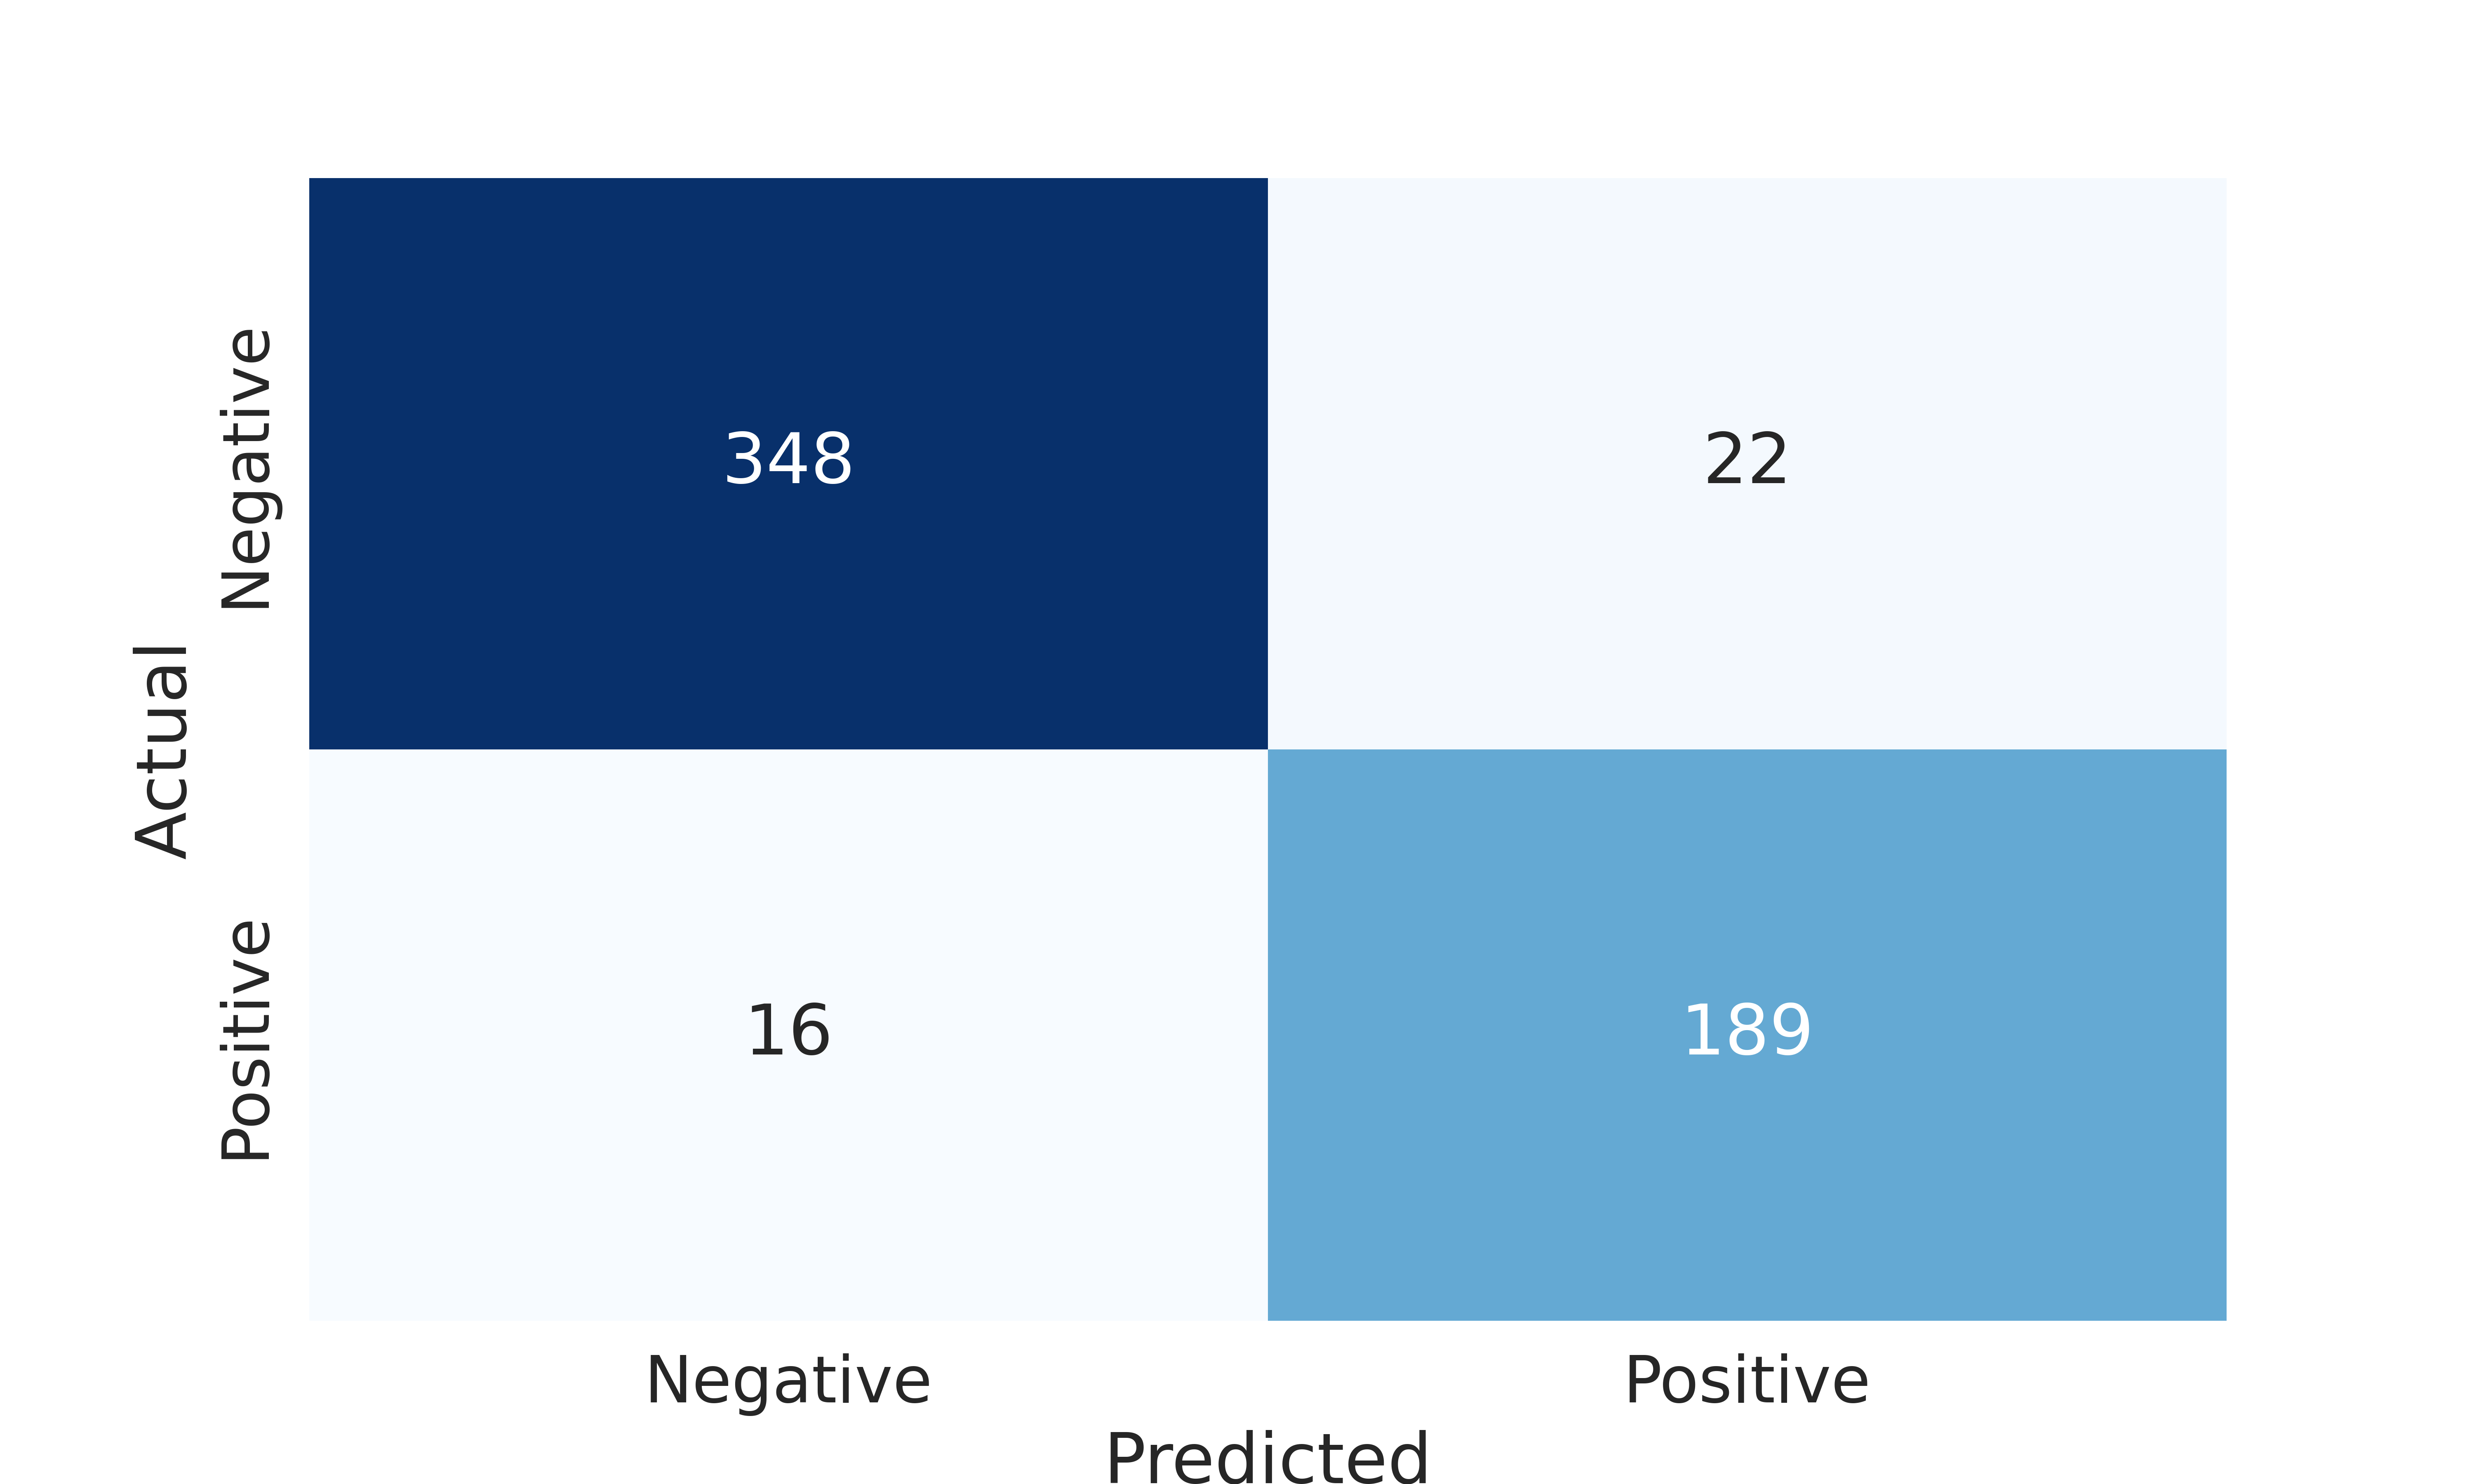
\includegraphics[width=\linewidth]{figures/confusion_bertweet.png}
        \caption{BERTweet - Confusion Matrix}
    \end{subfigure}
    \hfil
    \begin{subfigure}{0.45\linewidth}
        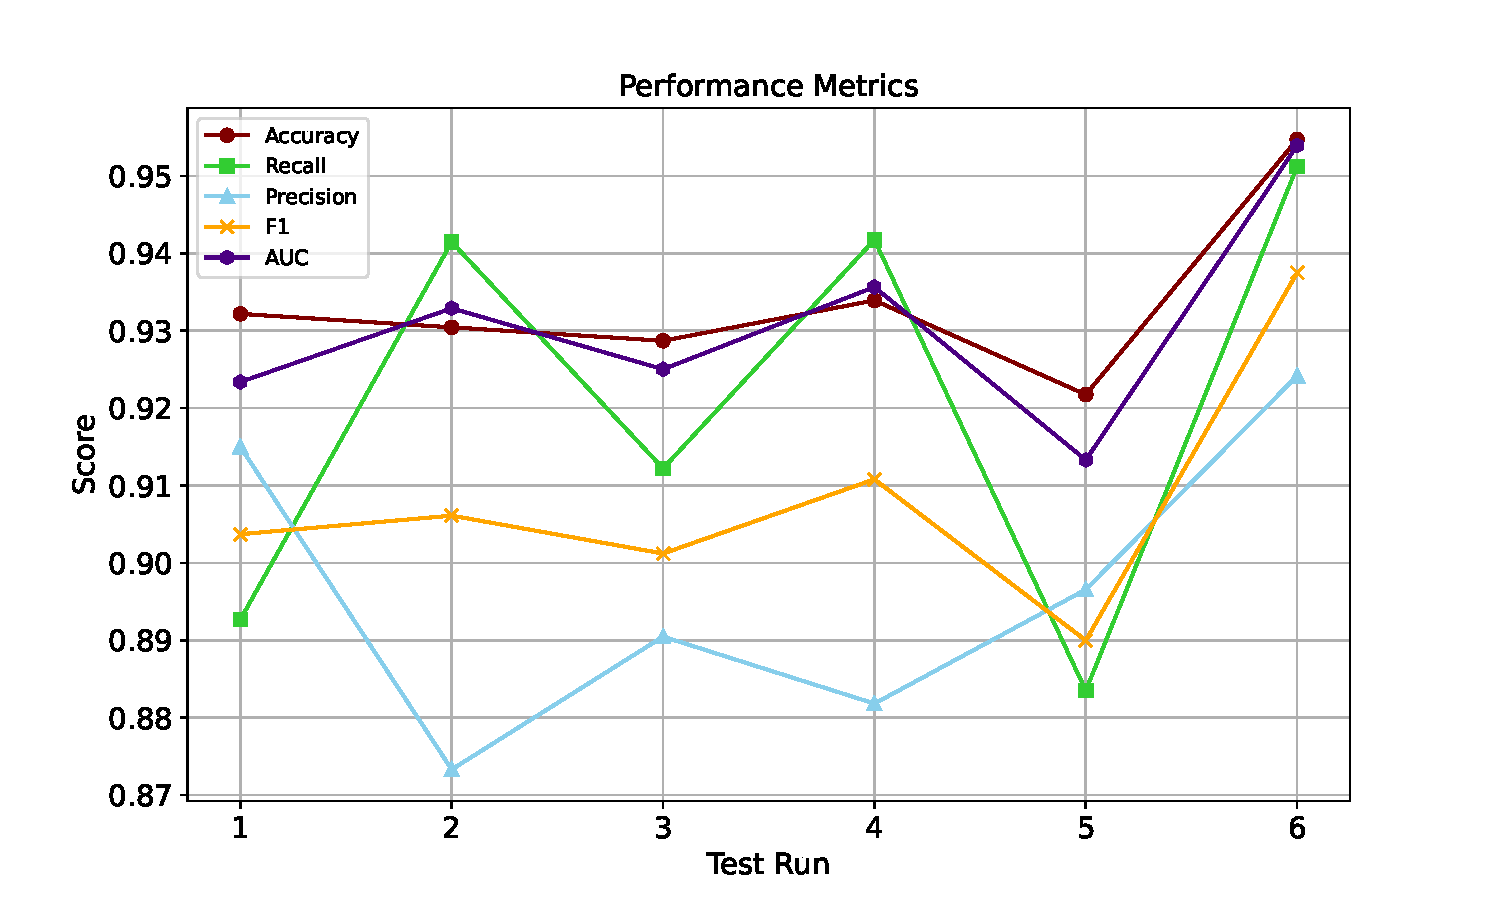
\includegraphics[width=\linewidth]{figures/metrics_line_bertweet.pdf}
        \caption{BERTweet - Performance Metrics}
    \end{subfigure}

    \begin{subfigure}{0.45\linewidth}
        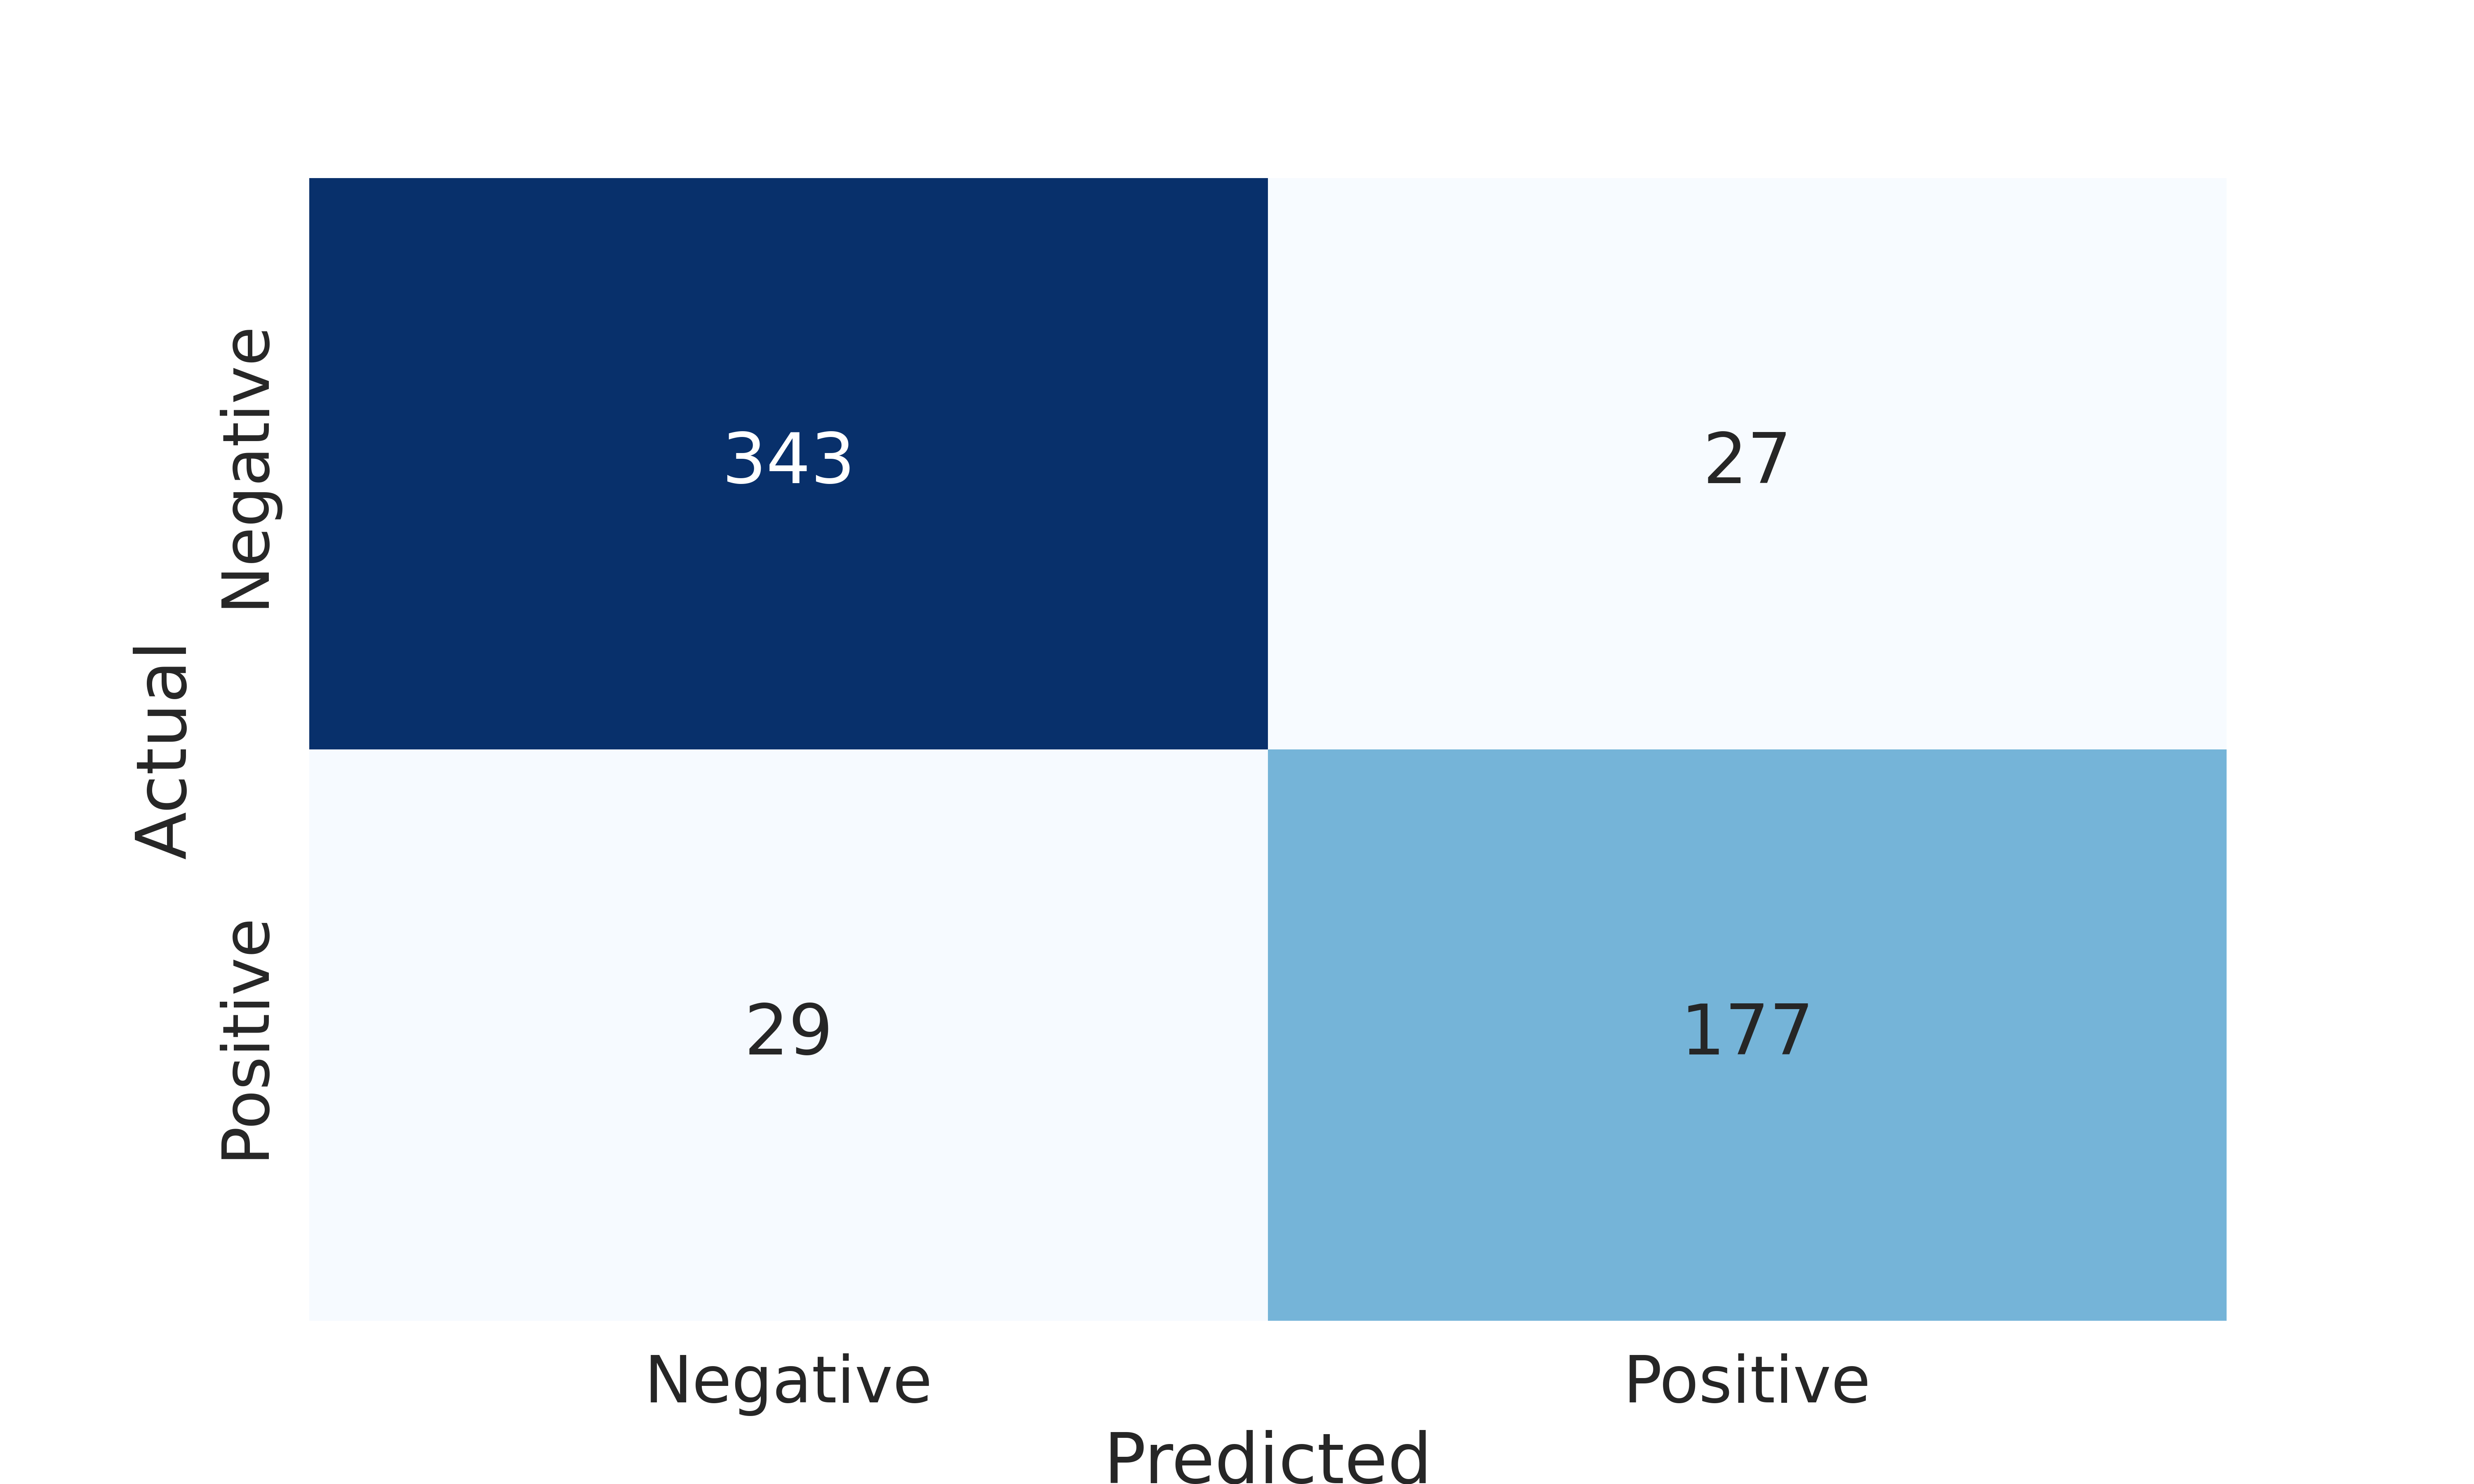
\includegraphics[width=\linewidth]{figures/confusion_distilbert.png}
        \caption{DistilBERT - Confusion Matrix}
    \end{subfigure}
    \hfil
    \begin{subfigure}{0.45\linewidth}
        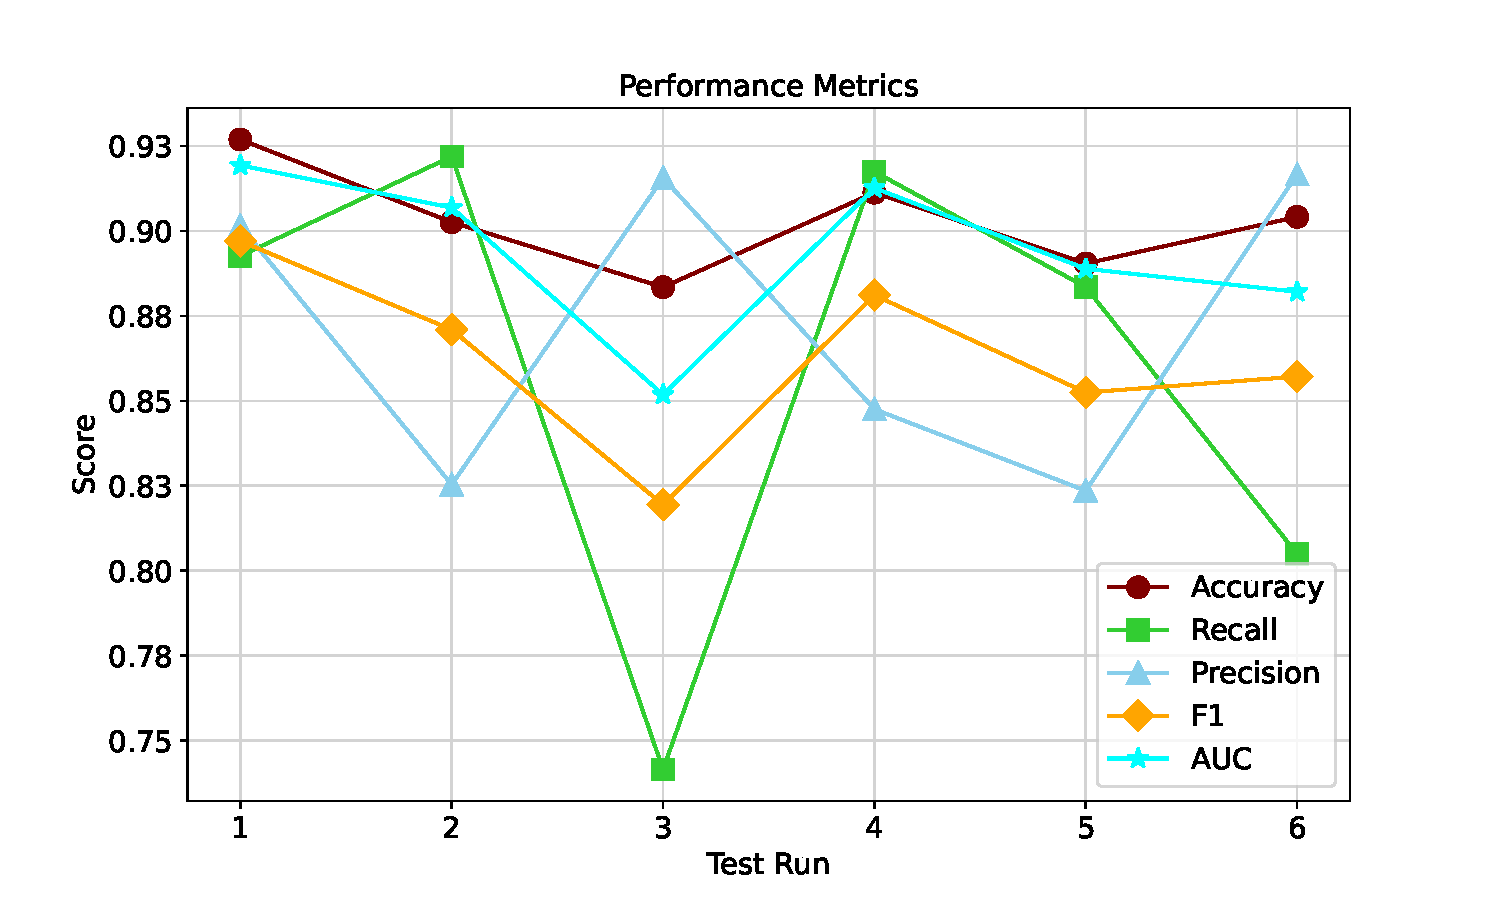
\includegraphics[width=\linewidth]{figures/metrics_line_distilbert.pdf}
        \caption{DistilBERT - Performance Metrics}
    \end{subfigure}

    \begin{subfigure}{0.45\linewidth}
        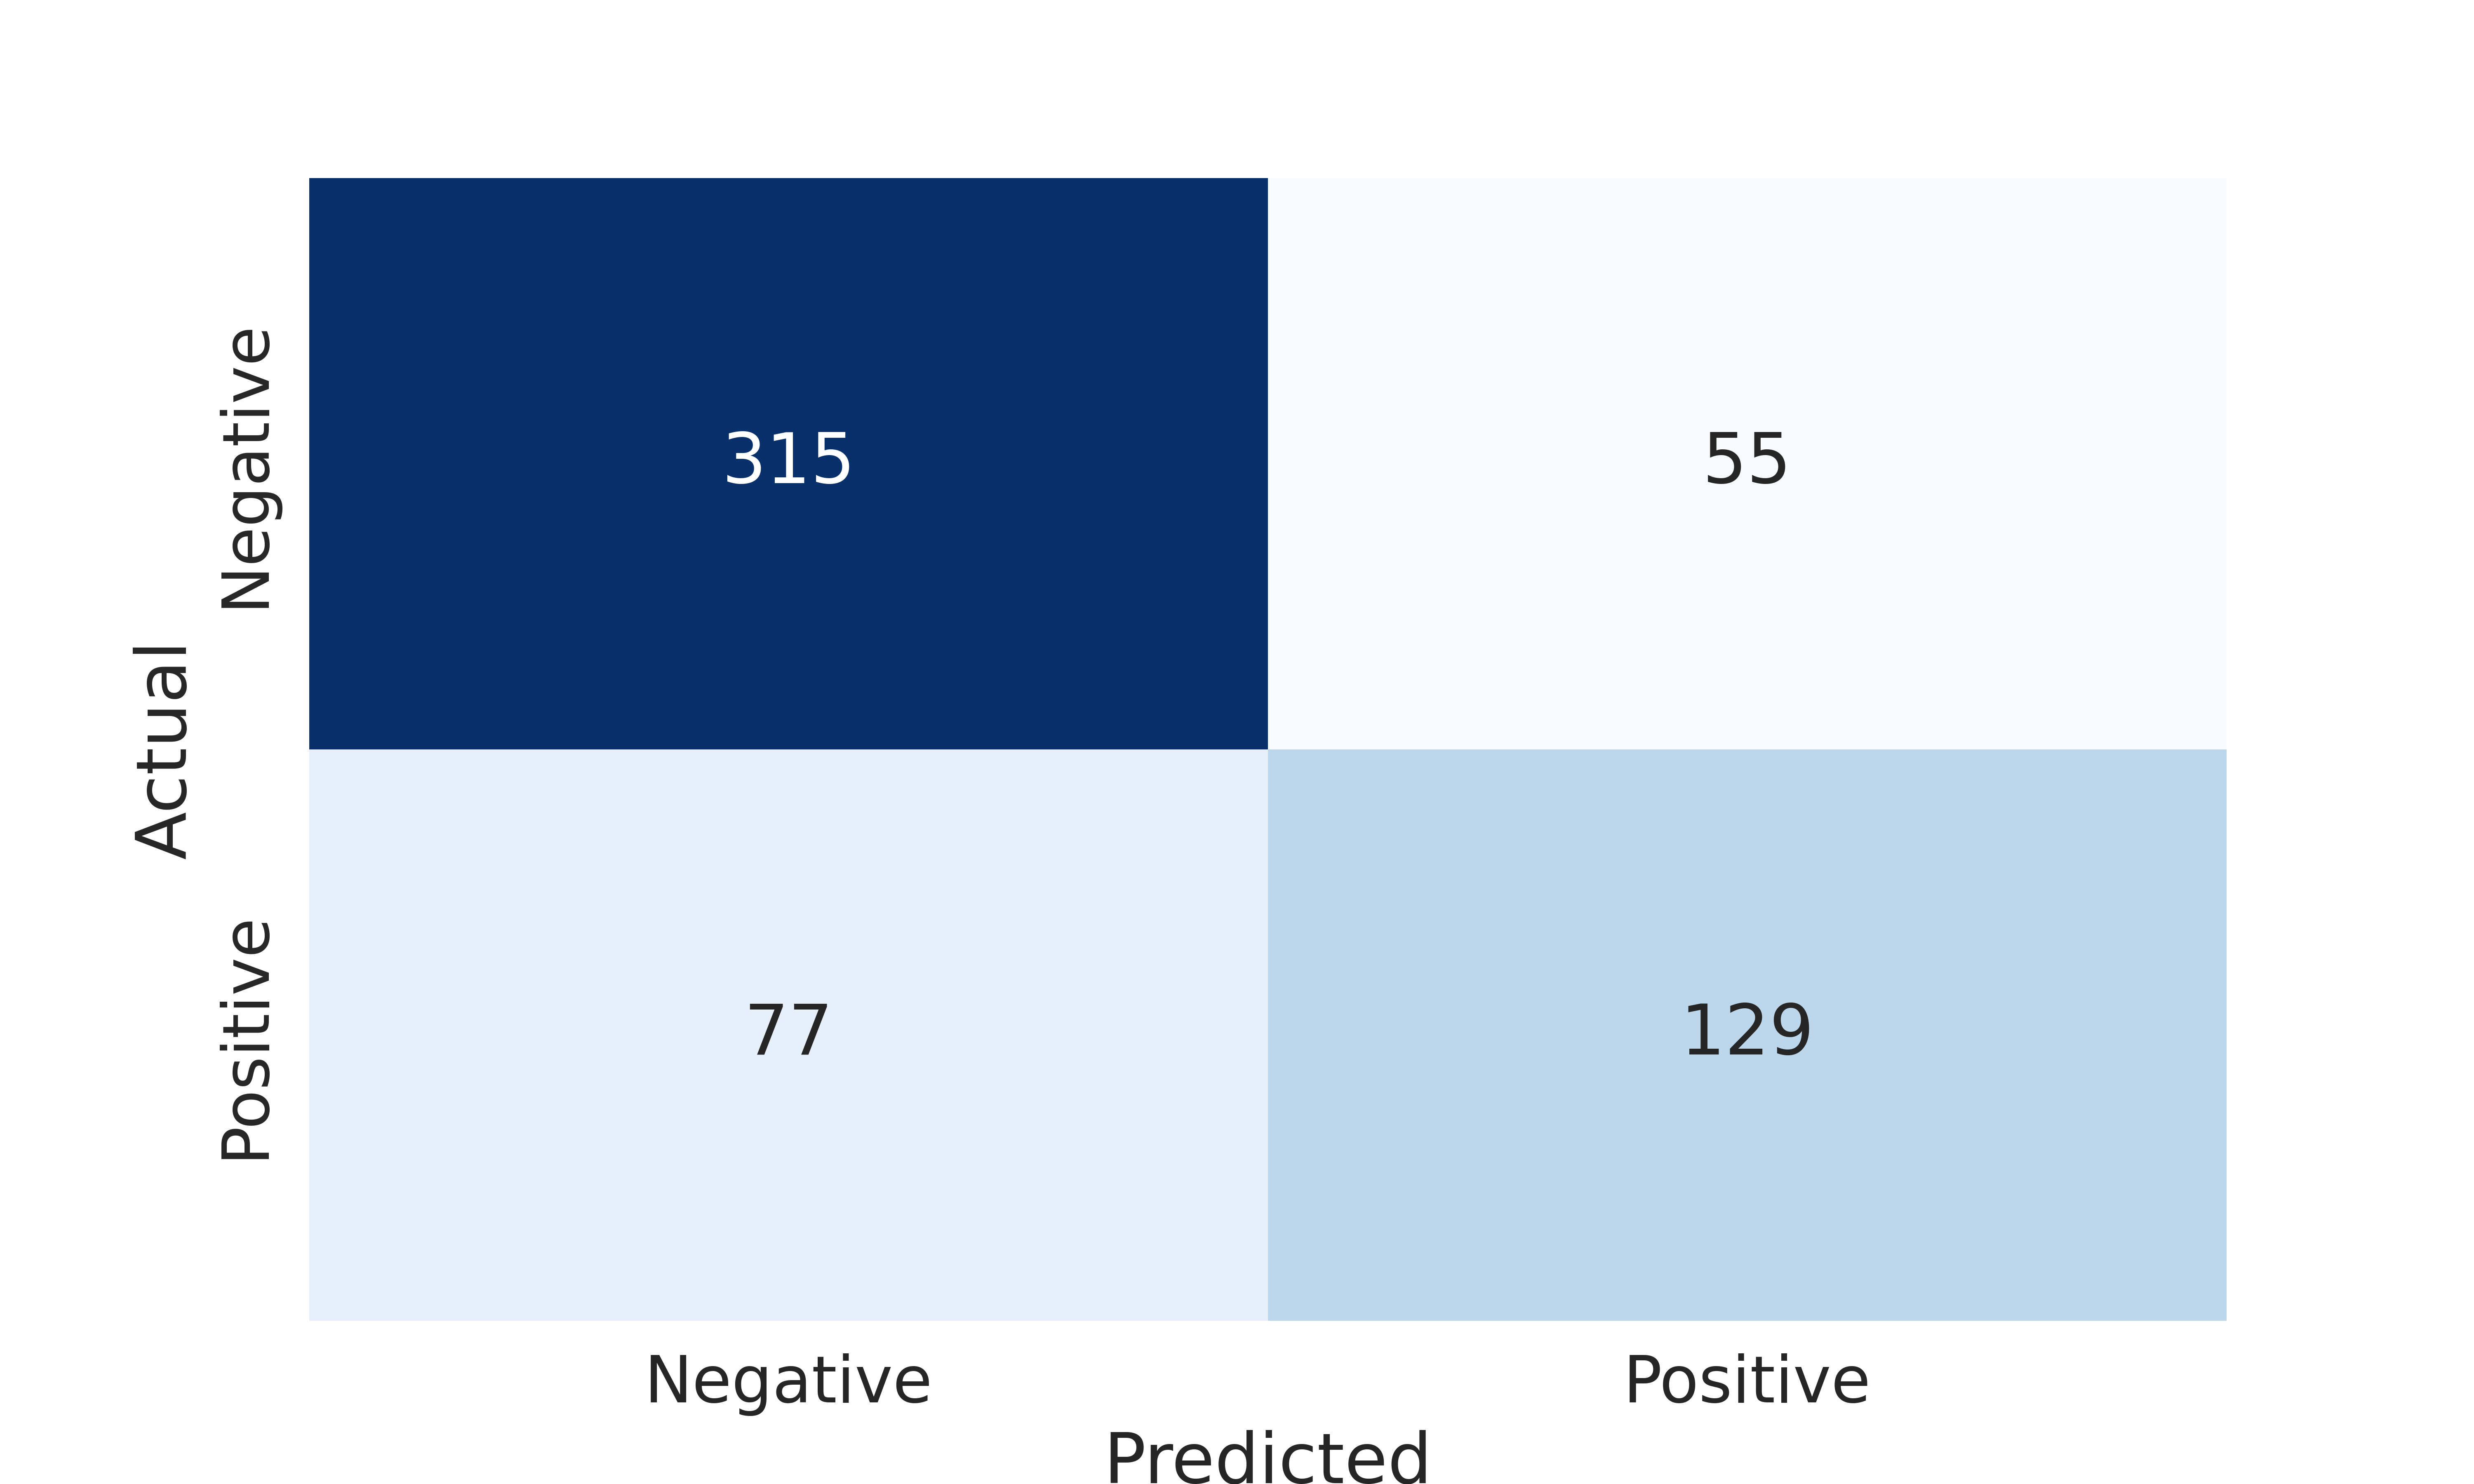
\includegraphics[width=\linewidth]{figures/confusion_berttiny.png}
        \caption{BERT Tiny - Confusion Matrix}
    \end{subfigure}
    \hfil
    \begin{subfigure}{0.45\linewidth}
        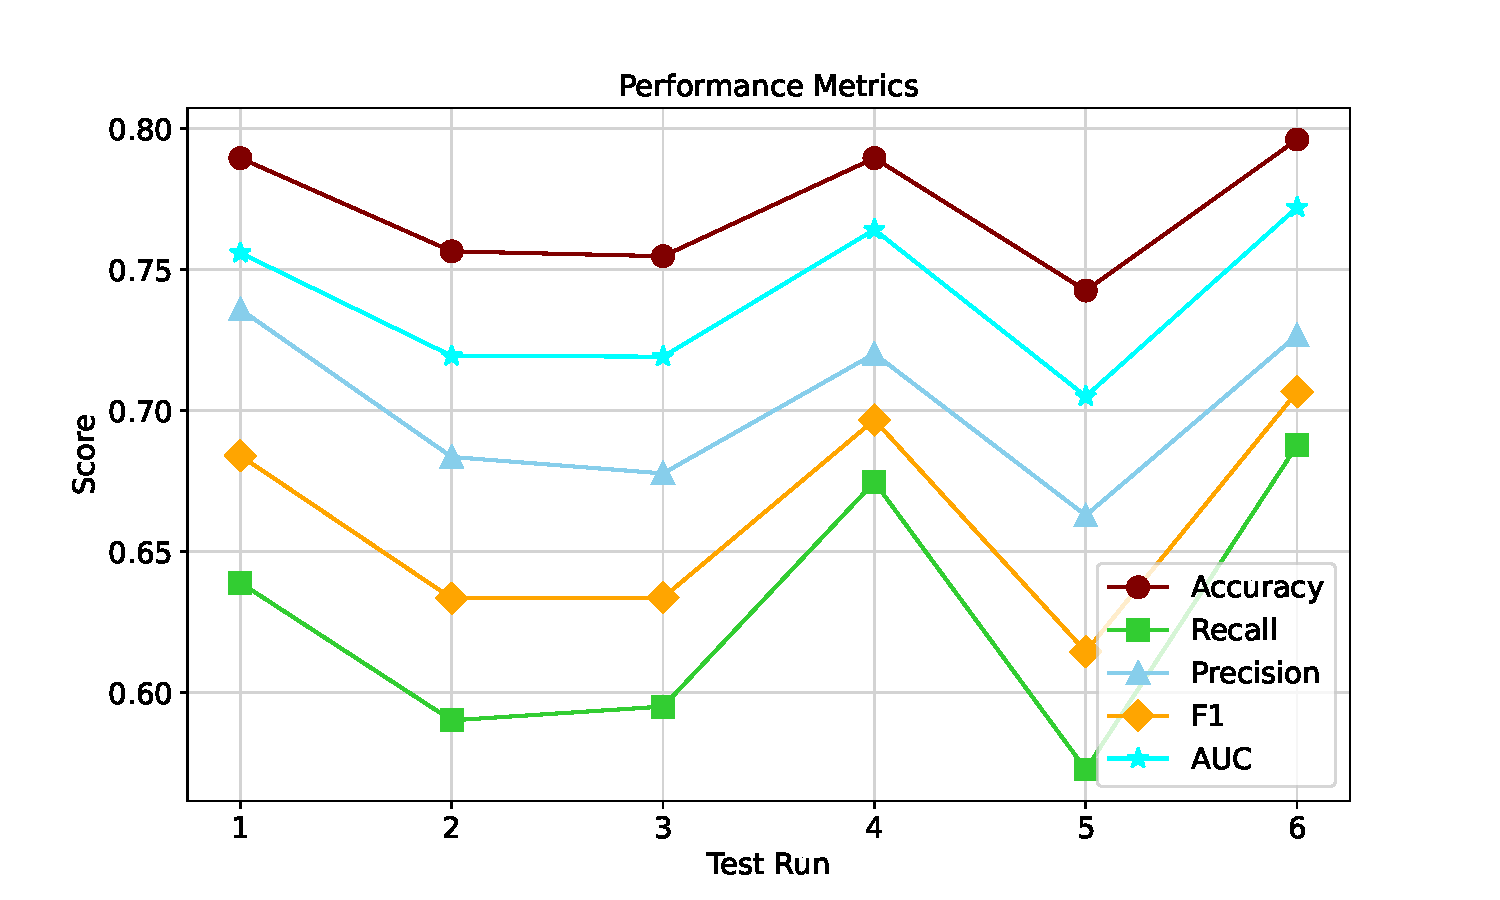
\includegraphics[width=\linewidth]{figures/metrics_line_berrttiny.pdf}
        \caption{BERT Tiny - Performance Metrics}
    \end{subfigure}
    \caption{Confusion matrix and performance metrics for the 3 selected models from the inference phase. The confusion matrix is based on the mean of values from the 6 outer loop iterations and the grid can be read from left to right as true negative, false positive, false negative and true positive.}
    \label{fig: deep_dive_results}
\end{figure}

The test losses for the 6 runs are given in Table \ref{tab: test_loss} while the graphs for the performance scores from inference are illustrated in Figure \ref{fig: deep_dive_results}. As expected, the test loss is lower for most the of 6 runs for BERTweet Base compared to the other two models. DistilBERT Base shows losses that are closer to BERT Base in 2 runs but otherwise are generally higher. There is a considerable difference for BERT Tiny which reflects in the predictive performance scores discussed earlier.\\

Referring to the metrics in Figure \ref{fig: deep_dive_results}, BERT Tiny exhibits a pattern that differs from the other 2 models. Based on the correct and incorrect classifications for all the inference executions (detailed in \ref{sec: conf_matrix_test_runs}), it appears that within each test run, the change in the misclassified complaint and non-complaint tweets move in the same direction. Another point to note is that BERTweet and DistilBERT seem to have relatively high fluctuations in recall and precision, likely due to inherent variations in the data splits from the cross-folds for each run. Considering the class imbalance, the analysis includes evaluating the ROC AUC scores. BERTweet demonstrates superior discrimination capability compared to the other two models, as reflected in its AUC score while exhibiting the least variability with a standard deviation of 0.01. DistilBERT has the next best score but displays slightly greater variance with a standard deviation of 0.02. In contrast, BERT Tiny showcases the lowest AUC scores and the highest standard deviation at 0.03.\\

Figure \ref{fig: deep_dive_results} also shows the confusion matrices for the 3 models based on the mean of the classifications from the 6 test runs. The ratio of accurately categorized non-complaint tweets (true negatives) to complaint tweets (true positives) is comparable between BERTweet and DistilBERT, but it's lower for BERT Tiny. All models appear to face greater challenges in accurately classifying complaint tweets compared to non-complaint tweets, although BERTWeet has the best recall scores overall. Even though there is an inherent class imbalance in the dataset, the confusion matrix and the metrics presented still offer valuable insights into the predictive capabilities of the models\\

Next, an error analysis is conducted on the tweets that were misclassified. Sample tweets that were inaccurately classified by the three models are presented in Table \ref{tab: error_tweets}. Examining tweets that were wrongly labelled as non-complaints several observations are discussed. BERTweet seems to have challenges in identifying acts of complaining which include the usage of very concise text (example 1) or very limited context (example 2). DistilBERT is unable to identify the use of sarcasm (example 5) and the usage of rhetorical questions (example 6). Notably, BERT Tiny struggles even when tweets exhibit multiple indicators of complaining, as seen in examples 9 and 10. Regarding tweets that were erroneously classified as complaints, the potential reasons are more difficult to speculate on. There are tweets containing words commonly associated with grievances, like 'waiting' and 'issue' (examples 3 and 4 for BERTweet) which is possibly confusing the model. DistilBERT misclassifies tweets that narrate negative experiences rather than expressing complaints (example 7) as well as instances where the text represents an intermediate segment of a conversation (example 8). In the case of the latter, while there is a hint of complaining it is not an act of complaining in this context. BERT Tiny appears to get confused when encountering text containing questions that carry no hint of complaining and are about mundane topics (examples 11 and 12). There possibly could be improvements to be found if more examples of such scenarios are included in the data used for finetuning, especially for the BERTweet and DistilBERT models. 

% error analysis tweets
\begin{table}
    \small
    \centering
    \begin{tblr}{
        width = \linewidth,
        colspec = {Q[35]Q[908]},
        row{1} = {Nobel,c},
        row{2} = {c},
        row{5} = {Mercury},
        row{6} = {Mercury},
        row{7} = {c},
        row{10} = {Mercury},
        row{11} = {Mercury},
        row{12} = {c},
        row{15} = {Mercury},
        row{16} = {Mercury},
        cell{2}{1} = {c=2}{0.943\linewidth},
        cell{7}{1} = {c=2}{0.943\linewidth},
        cell{12}{1} = {c=2}{0.943\linewidth},
        hlines,
        vlines,
        }
        \textbf{No.}        & \textbf{Tweet}\\
        \textbf{BERTweet}   & \\
        1                   & worst *\\
        2                   & . <user> <user> cuda driver lion update , please ? <url>\\
        3                   & i had entered in giveway contest for oneplus 5t lava . so waiting for the result\\
        4                   & i just checked again and i'm not having the same issues i had earlier . thanks for the help\\
        \textbf{DistilBERT} & \\
        5                   & just want to thank <user> <user> for ignoring me for three days xxxx\\
        6                   & is this really what you call a large milkshake <user> <url>\\
        7                   & shout out to the social media team <user> <user> whilst i get the frustration , there's never a time people should be insulting or rude when tweeting . these good people responding are employee's just tyring to help . \#heathrowairport \#heathrow \#britishairways \\
        8                   & no , see screenshot . it's the app . i got it straight off the playstore on android .\\
        \textbf{BERT Tiny}  &\\
        9                   & whyyyy is your wifi so slow <user> ?\\
        10                  & my 2nd visit to kfc chadwell heath after the last fiasco . this time they had no gravy or corn  amp ; forgot my chips \#fail\\
        11                  & is it possible to integrate my medium account on my personal website with your api ?\\
        12                  & thanks for your response . what is the twitter handle for your care centre in delhi , india ?
    \end{tblr}
    \caption{Sample tweets which have been misclassified by the 3 selected models. Tweets in the \colorbox{Mercury}{lighter shade of grey} are misclassified as complaints while the rest are misclassified as not complaints.}
    \label{tab: error_tweets}
\end{table}


\section{Experiment set 2 results: Cross-domain results}
% Cross domain results table
\begin{table}
    \centering
    \resizebox{\linewidth}{!}{%
        \begin{tblr}{
            row{odd} = {Mercury},
            row{1} = {Nobel},
            cell{2}{2} = {c},
            cell{2}{3} = {c},
            cell{2}{4} = {c},
            cell{2}{5} = {c},
            cell{2}{6} = {c},
            cell{2}{7} = {c},
            cell{2}{8} = {c},
            cell{2}{9} = {c},
            cell{2}{10} = {c},
            cell{3}{2} = {c},
            cell{3}{3} = {c},
            cell{3}{4} = {c},
            cell{3}{5} = {c},
            cell{3}{6} = {c},
            cell{3}{7} = {c},
            cell{3}{8} = {c},
            cell{3}{9} = {c},
            cell{3}{10} = {c},
            cell{4}{2} = {c},
            cell{4}{3} = {c},
            cell{4}{4} = {c},
            cell{4}{5} = {c},
            cell{4}{6} = {c},
            cell{4}{7} = {c},
            cell{4}{8} = {c},
            cell{4}{9} = {c},
            cell{4}{10} = {c},
            cell{5}{2} = {c},
            cell{5}{3} = {c},
            cell{5}{4} = {c},
            cell{5}{5} = {c},
            cell{5}{6} = {c},
            cell{5}{7} = {c},
            cell{5}{8} = {c},
            cell{5}{9} = {c},
            cell{5}{10} = {c},
            cell{6}{2} = {c},
            cell{6}{3} = {c},
            cell{6}{4} = {c},
            cell{6}{5} = {c},
            cell{6}{6} = {c},
            cell{6}{7} = {c},
            cell{6}{8} = {c},
            cell{6}{9} = {c},
            cell{6}{10} = {c},
            cell{7}{2} = {c},
            cell{7}{3} = {c},
            cell{7}{4} = {c},
            cell{7}{5} = {c},
            cell{7}{6} = {c},
            cell{7}{7} = {c},
            cell{7}{8} = {c},
            cell{7}{9} = {c},
            cell{7}{10} = {c},
            cell{8}{2} = {c},
            cell{8}{3} = {c},
            cell{8}{4} = {c},
            cell{8}{5} = {c},
            cell{8}{6} = {c},
            cell{8}{7} = {c},
            cell{8}{8} = {c},
            cell{8}{9} = {c},
            cell{8}{10} = {c},
            cell{9}{2} = {c},
            cell{9}{3} = {c},
            cell{9}{4} = {c},
            cell{9}{5} = {c},
            cell{9}{6} = {c},
            cell{9}{7} = {c},
            cell{9}{8} = {c},
            cell{9}{9} = {c},
            cell{9}{10} = {c},
            cell{10}{2} = {c},
            cell{10}{3} = {c},
            cell{10}{4} = {c},
            cell{10}{5} = {c},
            cell{10}{6} = {c},
            cell{10}{7} = {c},
            cell{10}{8} = {c},
            cell{10}{9} = {c},
            cell{10}{10} = {c},
            cell{11}{2} = {c},
            cell{11}{3} = {c},
            cell{11}{4} = {c},
            cell{11}{5} = {c},
            cell{11}{6} = {c},
            cell{11}{7} = {c},
            cell{11}{8} = {c},
            cell{11}{9} = {c},
            cell{11}{10} = {c},
            vlines,
            hline{1-2,11-12} = {-}{},
                    hline{3} = {2-10}{white},
                }
            \diagbox{\textbf{Train}}{\textbf{Test}} & \textbf{Food}  & \textbf{Appr. } & \textbf{Cars } & \textbf{Retail } & \textbf{Srvcs. } & \textbf{Softw. } & \textbf{Trans. } & \textbf{Elect. } & \textbf{Other } \\
            \textbf{Food}   & -         & 0.515 0.714          & 0.522 0.847         & 0.528 0.774           & 0.532 0.765           & \textbf{0.534} 0.797  & 0.517 0.718           & 0.529 0.762           & 0.510 \textbf{0.855}          \\
            \textbf{Appr.}  & \textbf{0.854} \textbf{0.918} & -          & 0.775 0.901         & 0.828 0.864           & 0.807 0.860           & 0.852 0.880           & 0.801 0.840           & 0.795 0.856           & 0.830 0.916          \\
            \textbf{Cars}         & 0.500 0.840         & 0.500 0.713          & -              & 0.500 0.765          & 0.500 0.757           & 0.500 0.789           & 0.500 0.717           & 0.500 0.755           & 0.500 \textbf{0.852}          \\
            \textbf{Retail} & \textbf{0.798} \textbf{0.889} & 0.706 0.788          & 0.715 0.888         & -           & 0.698 0.812           & 0.752 0.869           & 0.698 0.787           & 0.701 0.821           & 0.666 0.889          \\
            \textbf{Srvcs.} & 0.820 0.804         & 0.829 0.821          & 0.781 0.860         & 0.812 0.817           & -             & 0.834 0.856           & 0.802 0.811           & 0.824 0.852           & \textbf{0.885} \textbf{0.913} \\
            \textbf{Softw.} & \textbf{0.789} 0.848 & 0.761 0.809          & 0.747 0.901         & 0.786 0.852           & 0.738 0.838           & -            & 0.736 0.806           & 0.757 0.845           & 0.748 \textbf{0.906}          \\
            \textbf{Trans.} & 0.853 0.859         & 0.813 0.819          & 0.800 0.898         & 0.833 0.856           & 0.807 0.854           & 0.840 0.876           & -             & 0.777 0.825           & \textbf{0.871} \textbf{0.915} \\
            \textbf{Elect.} & 0.825 0.842         & 0.834 0.839          & 0.813 0.896         & 0.847 0.856           & 0.825 0.876           & \textbf{0.853} 0.891  & 0.790 0.812           & -                & 0.843 \textbf{0.919}       \\
            \textbf{Other}  & 0.500 0.840         & 0.500 0.713          & 0.500 \textbf{0.845}         & 0.500 0.765           & 0.500 0.757           & 0.500 0.789           & 0.500 0.717           & 0.500 0.755           & -            \\
            \textbf{All}    & 0.870 0.869         & 0.856 0.871          & 0.837 0.903        & 0.879 0.889          & 0.851 0.874          & 0.882 0.905          & 0.824 0.829           & 0.838 0.848           & \textbf{0.908} \textbf{0.951}
        \end{tblr}
    }
    \caption{ROC-AUC and F1 scores for the cross-domain experiments are recorded here. The rows show the domain used for finetuning while the columns represent the domains used for testing. The last row shows the scores where the full data except the corresponding test domain was used for finetuning. Best scores where applicable are highlighted in bold.}
    \label{tab: cross_domain_results}
\end{table}
What follows are the results from the cross-domain experiments. To recap, these experiments aim to evaluate the behaviour of the top-performing model from experiments set 1 in the context of smaller datasets and imbalanced class distributions. For these experiments, the chosen model is BERTweet Base, utilizing the optimal learning rate hyperparameter of 0.00003. The outcomes are detailed in Table \ref{fig: cross_domain_heat}, focusing on the assessment performed using ROC-AUC and F1 scores. The AUC metric is included due to its appropriateness for datasets with class imbalance. The metrics are reported as the mean of 3 test runs based on a stratified cross-fold split of the data. For a comprehensive breakdown of classes within each domain, please refer to Section \ref{sec: apdxa_fulldataset}.\\

The best performance is where all the data except the 'Other' domain tweets is used for finetuning and the 'Other' domain for testing. It has a relatively high discriminative ability represented by an AUC score of 0.908. Moreover, the achieved F1 score of 0.951 indicates a good balance between its precision and recall as well. The use of diverse domains for finetuning likely has a positive impact on how the models learn for the downstream task. In general, the predictive performance of the experiments where all data except one domain is used for finetuning is consistently higher when compared to using just a single domain for finetuning.\\

For single-domain finetuning cases, some instances exhibit performance levels approaching those attained through finetuning with the entire dataset, even though the volume of training data is significantly lower. Domains such as 'Apparel', 'Services', 'Transport' and 'Electronics' have AUC and F1 scores of over 0.8 despite the volume of data being on average only 10\% of the 'All' data volume. However, it's also important to highlight that finetuning with single domains with extremely limited data for finetuning results in AUC scores around or close to 0.5. This indicates that the model's predictive ability is akin to random chance in these cases. These include the domains of Cars', 'Food \& beverage', and 'Others' with only 4\% of the 'All' data volume on average. This is similar to the observations from \cite{jin_complaint_2020}. In the overall context, the notable performance of  'Food' and 'Other' as testing domains should be approached with caution, given the limited amount of inference data available.\\

The best score achieved by the previous baseline \cite{jin_complaint_2020} using BERT Base was 0.882 when employing all domains for finetuning and the 'Other' domain for testing. While BERTweet's best performance is for the same combination, the F1 score is significantly higher at 0.951. This notable difference in performance can likely be attributed to the advantages previously outlined for BERTweet Base, which is pre-trained on Twitter data. The predictive performance when finetuning with domains with very low tweet volumes is also higher for BERTweet. For the 'Cars' domain, which uses the lowest volume of data, BERT Base scores an average F1 of 0.623 while BERTweet achieves a substantially higher F1 of 0.774.\\

% cross domain heatmap
\begin{figure}[htb]
    \centering
    \captionsetup{font=small}
    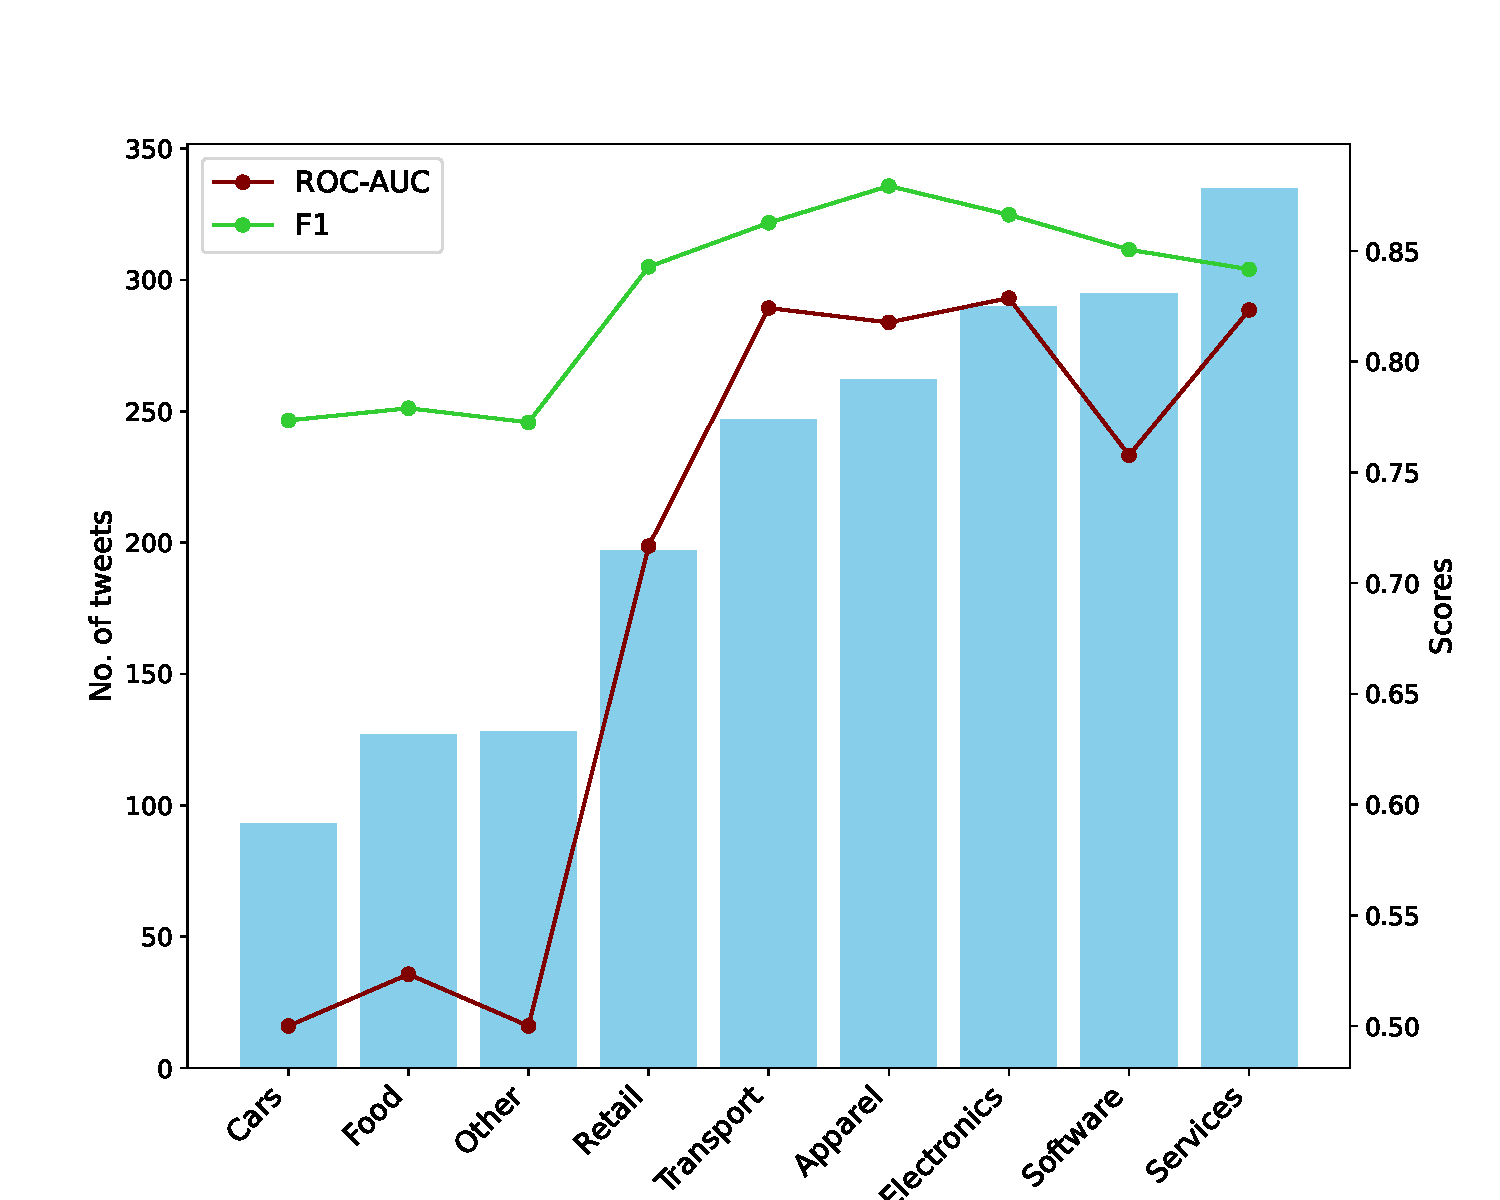
\includegraphics[width=12cm]{figures/cross_domain_instancevsmetric.pdf}
    \vspace*{-3mm}
    \caption{Shows a plot of the number of tweets for each domain against the average performance when that domain is used for finetuning.}
    \label{fig: cross_domain_train_domain}
\end{figure}

Continuing to explore the relationship between the volume of data and the performance, Figure \ref{fig: cross_domain_train_domain} illustrates the impact of the number of instances or tweets utilized during the finetuning process on the average testing performance. Additionally, it shows the breakdown of complaint and non-complaint tweets. At a macro level, it appears the predictive performance improves as the volume of data available for finetuning increases. However, specific domains like 'Other', 'Apparel', and 'Software' exhibit deviations from this trend. Inherent characteristics of tweets within these domains could be influencing their performance deviations. All domains predominantly feature complaints as the dominant class. However, no distinct pattern emerges from how the variations in the class imbalance impact performance in this situation.
\chapter{Conclusions}

With the advancement of technology and the widespread adoption of social media, the anticipated response times for businesses to address complaints have significantly reduced. Furthermore, this evolution has introduced numerous online avenues through which customers can seek assistance or voice their grievances. These platforms grant substantial visibility, thereby exposing organizations to the effects of negative online word of mouth. Consequently, the implementation of tools to automatically detect complaints has many benefits for organisations.\\

Building upon earlier research in this field, this study has led to a few key conclusions. First and foremost, it's apparent that BERTweet outperforms the other assessed transformer models in identifying complaints within Twitter streams. Nevertheless, it's advisable to exercise caution when generalizing this finding to other platforms like Facebook, given the constraints of the pre-training data (limited to Twitter data). Notably, BERTweet shows comparatively good performance even when dealing with limited finetuning data. Additionally, a significant takeaway is that organizations constrained by memory and computational resources can effectively opt for smaller models like DistilBERT without significantly compromising predictive performance.\\

In conclusion, there exist several promising paths for further exploration within this research domain. Analyzing the performance of similar models on alternative social media platforms like Facebook could yield deeper insights into the models' capabilities on linguistically diverse datasets. Another avenue of potential interest involves evaluating the multi-modal approach with the BERTweet model and if the inclusion of additional linguistic cues could enhance its performance. Lastly, considering the ongoing advancements in generative models, exploring prompting with solutions that use state-of-the-art models like GPT 3.5 / 4 could have great value.


%\setlength{\parskip}{0pt} % NSM - reset single line space

\bibliographystyle{acm} 
\bibliography{mybibliography} 

\begin{appendices}
\chapter{Other supporting analysis and graphs}

\section{Breakdown of tweets in full dataset}
\label{sec: apdxa_fulldataset}
\begin{table}[ht]
    \captionsetup{font=small}
    \small
    \centering
    \begin{tabularx}{\textwidth}{|X|c|c|c|}
        \hline
        \rowcolor[gray]{0.7}
        \textbf{Domains}            & \textbf{Complaints}            & \textbf{Non-Complaints}        & \textbf{Total Tweets} \\
        \hline
        Apparel                     & 145 \small{(55.3\%)}           & 117 \small{(44.7\%)}           & 262 \small{(7.6\%)}   \\
        \hline
        Cars                        & 68 \small{(73.1\%)}            & 25 \small{(26.9\%)}            & 93 \small{(2.7\%)}    \\
        \hline
        Electronics                 & 176 \small{(60.7\%)}           & 114 \small{(39.3\%)}           & 290 \small{(8.4\%)}   \\
        \hline
        Food \& Beverage            & 92 \small{(72.4\%)}            & 35 \small{(27.6\%)}            & 127 \small{(3.7\%)}   \\
        \hline
        Other                       & 95 \small{(74.2\%)}            & 33 \small{(25.8\%)}            & 128 \small{(3.7\%)}   \\
        \hline
        Retail                      & 122 \small{(61.9\%)}           & 75 \small{(38.1\%)}            & 197 \small{(5.7\%)}   \\
        \hline
        Services                    & 204 \small{(60.9\%)}           & 131 \small{(39.1\%)}           & 335 \small{(9.7\%)}   \\
        \hline
        Software \& Online Services & 192 \small{(65.1\%)}           & 103 \small{(34.9\%)}           & 295 \small{(8.6\%)}   \\
        \hline
        Transport                   & 138 \small{(55.9\%)}           & 109 \small{(44.1\%)}           & 247 \small{(7.2\%)}   \\
        \hline
        \rowcolor[gray]{0.9}
        \textbf{Sub-total}          & \textbf{1232 \small{(62.4\%)}} & \textbf{742 \small{(37.6\%)}}  & \textbf{1974}         \\
        \hline
        \hline
        Random Reply                & 0 \small{(0\%)}                & 739 \small{(100\%)}            & 739 \small{(21.4\%)}  \\
        \hline
        Random Tweet                & 0 \small{(0\%)}                & 736 \small{(100\%)}            & 736 \small{(21.3\%)}  \\
        \hline
        \hline
        \rowcolor[gray]{0.9}
        \textbf{Total}              & \textbf{1232 \small{(35.7\%)}} & \textbf{2217 \small{(64.3\%)}} & \textbf{3449}         \\
        \hline
    \end{tabularx}
    \caption{The nine domains and the distribution of tweets that are complaints and those that are not from the latest version of the dataset available in the public domain and for the experiments. Additionally, the table includes the number of random tweets and replies introduced into the dataset by the authors for a more proportionate representation of the classes.}
    \label{tab: fulldataset_breakdown}
\end{table}

\section{Sample data from dataset}
\begin{table}[ht]
    \captionsetup{font=small}
    \small
    \centering
    \begin{tabularx}{\textwidth}{|l|X|c|c|l|}
        \hline
        \rowcolor[gray]{0.7}
        \textbf{id} & \textbf{text}                                               & \textbf{binarylabel} & \textbf{multilabel} & \textbf{domain} \\
        \hline
        1.20E+17    & asus g60 series . bought it to play games but guess not bf3 & 1                    & 1                   & electronics     \\
        \hline
        4.88E+17    & love this trimmer ! making the sidewalk look sharp <url>    & 0                    & 0                   & other           \\
        \hline
    \end{tabularx}
    \caption{Sample data from \cite{jinModelingSeverityComplaints2021}.}
    \label{tab: apdx_sample_data}
\end{table}

The \texttt{binarylabel} represents the label for complaints with 1 indicating the tweet is a complaint. Columns \texttt{id} and \texttt{multilabel} are not used for the experiments.



\section{Token distribution after tokenization}
\label{sec: apdxa_token_dist}
The graphs in Figure \ref{fig: apdxa_tokens} show the distribution of token size for tweets from the full dataset for each of the models based on the tokenizer they use. The graph for BERT base uncased is in Chapter 3, Figure \ref{fig: bef_aft_token}.
\begin{figure}[htbp]
    \centering
    \captionsetup{font=small}
    \begin{subfigure}[b]{0.48\textwidth}
        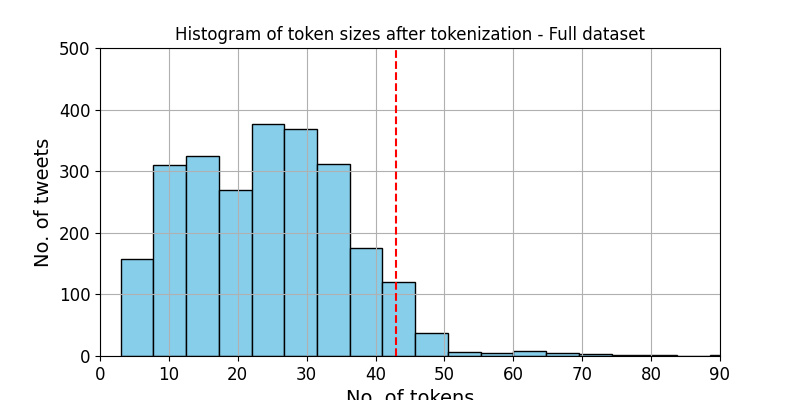
\includegraphics[width=\textwidth]{figures/token_pp_hist_albert-base-v2.png}
        \caption{AlBERT base}
        \label{fig: token_pp_hist_albert}
    \end{subfigure}
    \hfill
    \begin{subfigure}[b]{0.48\textwidth}
        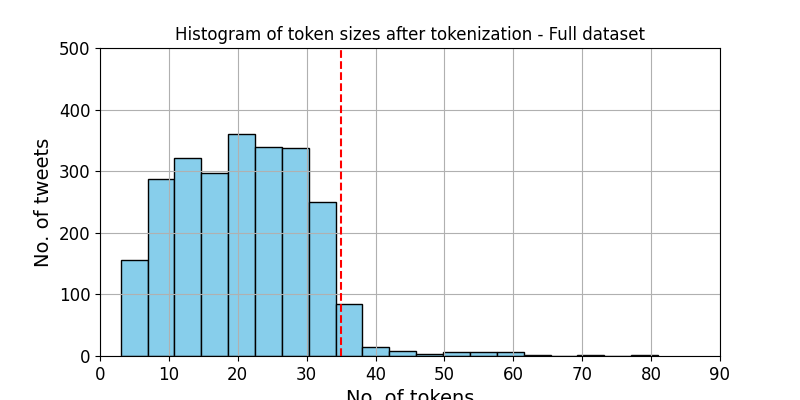
\includegraphics[width=\textwidth]{figures/token_pp_hist_vinai-bertweet-base.png}
        \caption{BERTweet}
        \label{fig: token_pp_hist_bertwteet}
    \end{subfigure}
    \begin{subfigure}[b]{0.48\textwidth}
        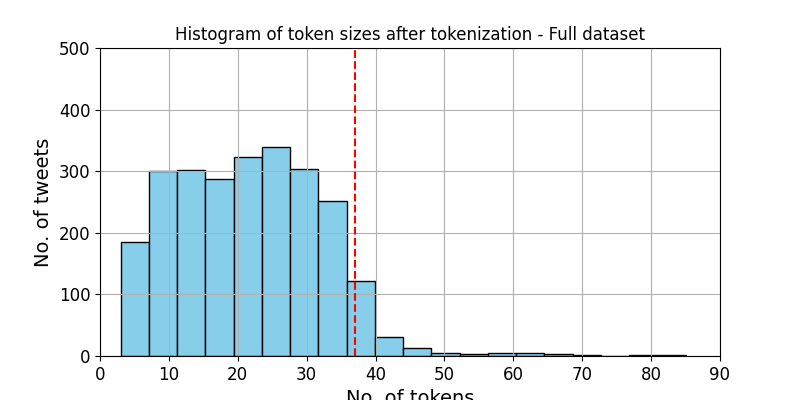
\includegraphics[width=\textwidth]{figures/token_pp_hist_prajjwal1-bert-tiny.png}
        \caption{BERT tiny}
        \label{fig: token_pp_hist_tiny}
    \end{subfigure}
    \hfill
    \begin{subfigure}[b]{0.48\textwidth}
        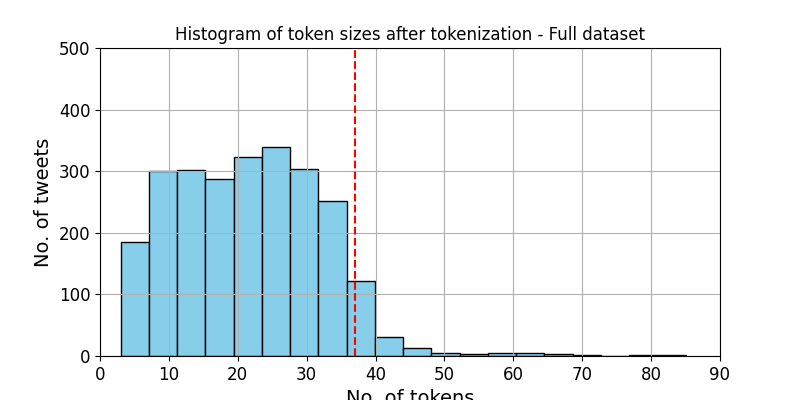
\includegraphics[width=\textwidth]{figures/token_pp_hist_distilbert-base-uncased.png}
        \caption{DistilBERT base uncased}
        \label{fig: token_pp_hist_distilbert}
    \end{subfigure}
    \begin{subfigure}[b]{0.48\textwidth}
        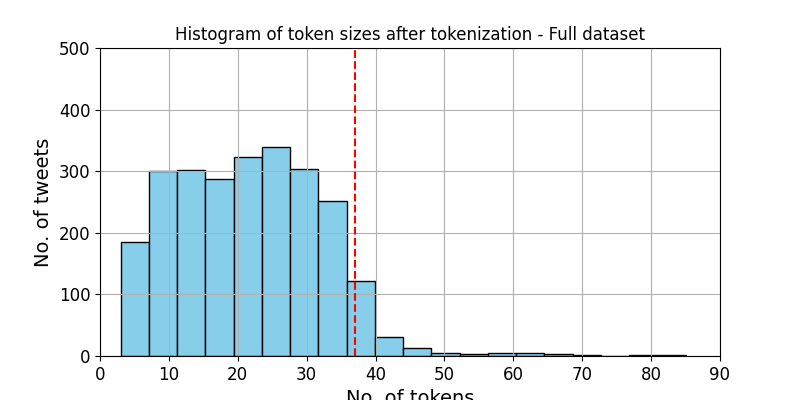
\includegraphics[width=\textwidth]{figures/token_pp_hist_google-mobilebert-uncased.png}
        \caption{MobileBERT uncased}
        \label{fig: token_pp_hist_mobile}
    \end{subfigure}
    \hfill
    \begin{subfigure}[b]{0.48\textwidth}
        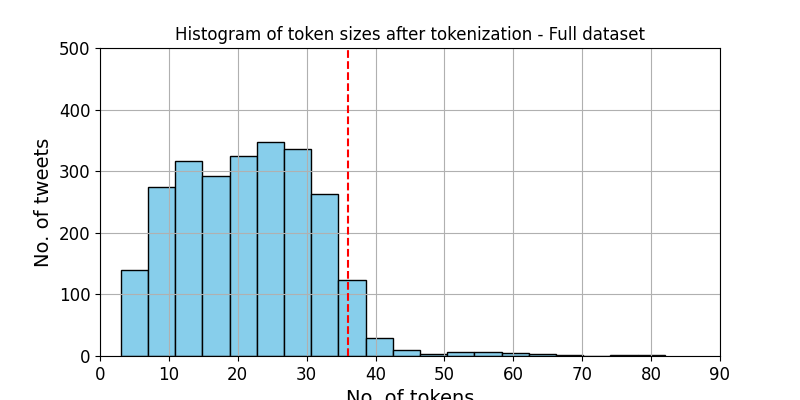
\includegraphics[width=\textwidth]{figures/token_pp_hist_roberta-base.png}
        \caption{RoBERTa base}
        \label{fig: token_pp_hist_roberta}
    \end{subfigure}
    \caption{The token count distribution for the full dataset of 3,449 tweets for all models.}
    \label{fig: apdxa_tokens}
\end{figure}

\subsection{Confusion matrix from every test run}
The elements of the matrix in left-to-right order are true negative, false positive, false negative and true positive.
\label{sec: conf_matrix_test_runs}
\begin{table}
    \centering
    \begin{tblr}{
      width = \linewidth,
      colspec = {Q[152]Q[283]Q[292]Q[194]},
      row{odd} = {Mercury},
      row{1} = {Nobel,c},
      column{1} = {c},
      cell{2}{2} = {c},
      cell{2}{3} = {c},
      cell{2}{4} = {c},
      cell{3}{2} = {c},
      cell{3}{3} = {c},
      cell{3}{4} = {c},
      cell{4}{2} = {c},
      cell{4}{3} = {c},
      cell{4}{4} = {c},
      cell{5}{2} = {c},
      cell{5}{3} = {c},
      cell{5}{4} = {c},
      cell{6}{2} = {c},
      cell{6}{3} = {c},
      cell{6}{4} = {c},
      cell{7}{2} = {c},
      cell{7}{3} = {c},
      cell{7}{4} = {c},
      hline{1-2,8} = {-}{},
      vlines,
    }
    \textbf{Test run} & \textbf{BERTweet Base}       & \textbf{DistilBERT Base}     & \textbf{BERT Tiny}           \\
    1                 & {{[}353~ ~17]\\{[} 22~ 183]} & {{[}350~ ~20]\\{[} 22~ 183]} & {{[}323~ ~47]\\{[} 74~ 131]} \\
    2                 & {{[}342~ ~28]\\{[} 12~ 193]} & {{[}330~ ~40]\\{[} 16~ 189]} & {{[}314~ ~56]\\{[} 84~ 121]} \\
    3                 & {{[}347~ ~23]\\{[} 18~ 187]} & {{[}356~ ~14]\\{[} 53~ 152]} & {{[}312~ ~58]\\{[} 83~ 122]} \\
    4                 & {{[}343~ ~26]\\{[} 12~ 194]} & {{[}335~ ~34]\\{[} 17~ 189]} & {{[}315~ ~54]\\{[} 67~ 139]} \\
    5                 & {{[}348~ ~21]\\{[} 24~ 182]} & {{[}330~ ~39]\\{[} 24~ 182]} & {{[}309~ ~60]\\{[} 88~ 118]} \\
    6                 & {{[}353~ ~16]\\{[} 10~ 195]} & {{[}354~ ~15]\\{[} 40~ 165]} & {{[}316~ ~53]\\{[} 64~ 141]} 
    \end{tblr}
    \caption{Confusion matrix from every test run for the experiments set 1.}
    \label{tab: conf_matrix_test_runs}    
\end{table}




\chapter{Other references}

\section{Additional information on environment used}
\begin{itemize}
    \small
    \item \textbf{CPU Model:} Intel Xeon Gold 5315Y Processor
    \item \textbf{Operating System:} Ubuntu 20.04.5 LTS
\end{itemize}

\section{References for transformer models used in experiment sets 1 and 2}
\begin{table}[ht]
    \captionsetup{font=small}
    \centering
    \begin{tabularx}{\textwidth}{|l|X|}
        \hline
        \rowcolor[gray]{0.7}
        \textbf{Model}            & \textbf{Model Documentation}                                   \\
        \hline

        AlBERT Base               & \small{\url{https://huggingface.co/albert-base-v2}}            \\
        \hline
        BERT Base (uncased)       & \small{\url{https://huggingface.co/bert-base-uncased}}         \\
        \hline
        BERT Tiny                 & \small{\url{https://huggingface.co/prajjwal1/bert-tiny}}       \\
        \hline
        BERTweet Base             & \small{\url{https://huggingface.co/vinai/bertweet-base}}       \\
        \hline
        DistilBERT Base (uncased) & \small{\url{https://huggingface.co/distilbert-base-uncased}}   \\
        \hline
        RoBERTa Base              & \small{\url{https://huggingface.co/roberta-base}}              \\
        \hline
    \end{tabularx}
    \caption{The transformer models used for the experiments and links to their documentation.}
    \label{tab: apdxb_model_doc}
\end{table}

\section{References for models used in data exploration}
Models used in the data exploration and analysis.
\begin{table}[ht]
    \captionsetup{font=small}
    \centering
    \begin{tabularx}{\textwidth}{|l|X|}
        \hline
        \rowcolor[gray]{0.7}
        \textbf{Model}                                   & \textbf{Model Documentation}                                                         \\
        \hline
        BERTweet base sentiment analysis (pysentimiento) & \small{\url{https://huggingface.co/finiteautomata/bertweet-base-sentiment-analysis}} \\
        \hline
    \end{tabularx}
    \caption{Sentiment analysis model and link to its documentation.}
    \label{tab: apdxb_other_model_doc}
\end{table}

\section{Evaluation metrics references}
\begin{table}[ht]
    \captionsetup{font=small}
    \centering
    \begin{tabularx}{\textwidth}{|l|X|}
        \hline
        \rowcolor[gray]{0.7}
        \textbf{Metric}                  & \textbf{Metric Documentation}                                                    \\
        \hline

        Accuracy                         & \small{\url{https://huggingface.co/spaces/evaluate-metric/accuracy}}             \\
        \hline
        F1                               & \small{\url{https://huggingface.co/spaces/evaluate-metric/f1}}                   \\
        \hline
        Precision                        & \small{\url{https://huggingface.co/spaces/evaluate-metric/precision}}            \\
        \hline
        Recall                           & \small{\url{https://huggingface.co/spaces/evaluate-metric/recall}}               \\
        \hline
        ROC AUC                          & \small{\url{https://huggingface.co/spaces/evaluate-metric/roc_auc}}              \\
        \hline
        Confusion Matrix                 & \small{\url{https://huggingface.co/spaces/BucketHeadP65/confusion_matrix}}       \\
        \hline
    \end{tabularx}
    \caption{The metrics used for evaluating the performance of the models in the experiments and links to their documentation.}
    \label{tab: apdxb_metric_doc}
\end{table}
\end{appendices}

\end{document}
